\documentclass[a4paper, 12pt]{article}
\usepackage[a4paper, total={6in, 8in}]{geometry}
\geometry{
	a4paper,
	left = 1.5 cm,
	right = 1.5 cm,
	top = 2cm,
	bottom = 2.5 cm,
}
\usepackage[T1]{fontenc}
\usepackage{pythontex}
\usepackage{hhline}
\usepackage{array,booktabs}
\newcolumntype{M}[1]{>{\centering\arraybackslash}m{#1}}
\usepackage[table]{xcolor}
\usepackage{caption}
\usepackage{makecell}
\usepackage{lipsum}
\usepackage{pifont}
\usepackage{amssymb}
\usepackage{amsmath}
\usepackage[utf8]{inputenc}
\usepackage[italian]{babel}
\usepackage{graphicx}
\graphicspath{ {./images/} }
\usepackage{spverbatim}
\usepackage{float}
\usepackage{url}
\usepackage{xstring}
\usepackage{hyperref}
\usepackage{xcolor}
\usepackage{upquote}
\definecolor{linkcolor}{RGB}{1,1,87}
\hypersetup{
    colorlinks,
    citecolor=black,
    filecolor=black,
    linkcolor=linkcolor,
    urlcolor=blue
}
\usepackage{fancyvrb,newverbs,xcolor}
\definecolor{cverbbg}{gray}{0.93}
\definecolor{cellcolor}{RGB}{165,194, 242}
\usepackage{xifthen}
\usepackage{multirow}
\usepackage{adjustbox}
\usepackage{listings}
\lstset{
  basicstyle=\ttfamily,
  backgroundcolor=\color{cverbbg},
  breaklines=true,
  frame=lines,
  framerule=1pt,
  numbers=left,
  numbersep=10pt, 
  keywordstyle=\color{blue},
  commentstyle=\color{green!60!black},
  stringstyle=\color{red},
  showstringspaces=false,  
  framextopmargin=1.5ex,
  framexbottommargin=1.5ex,
  framexleftmargin={\dimexpr 1.5em+3pt},
  xleftmargin={\dimexpr 1.5em+3pt},
  linewidth={\dimexpr \linewidth-3pt},
}

% following restart section enumeration in different \part
\usepackage{chngcntr}
\counterwithin*{section}{part}

\newcommand{\makesub}[1]{%
  \saveexpandmode\noexpandarg
  \StrSubstitute{#1}{\_}{_}[\temp]%
  \restoreexpandmode%
}

\newcommand{\target}[1]{%
  \makesub{#1}%
  \hypertarget{\temp}{}%
}

\newcommand{\attach}[1]{%
  \makesub{#1}%
  \hyperlink{\temp}{\emph{#1}}%
}
\newcommand{\attachcode}[1]{%
  \makesub{#1}%
  \hyperlink{\temp}{\code{#1}}%
}

\newcommand{\code}[1]{\colorbox{cverbbg}{	exttt{\detokenize{#1}}}}
%\newcommand{\code}[1]{\colorbox{cverbbg}{\texttt{\StrSubstitute{#1}{_}{\_}}}}

\newcommand{\linux}{\textit{Linux}}
\newcommand{\win}{\textit{Windows}}
\newcommand{\nota}[1]{\textbf{Nota}: #1}
\newcommand{\memo}[1]{\textbf{Memo}: #1}
\newcommand{\esempio}[1]{\textbf{Esempio}: #1}
\newcommand{\tbs}{\textbackslash}
\newcommand{\Null}{\code{NULL}}
\newcommand{\api}{\emph{API}}
\newcommand{\key}[1]{\texttt{\StrSubstitute{#1}{_}{\_}}}
\usepackage{eurosym}

\newcommand{\paramtable}[2][]{%
\ifthenelse{\isempty{#2}} {\input{|"/home/luca/latex_scripts/generate_param_table.py '#1'"}} {\input{|"/home/luca/Scrivania/MA/homeworks/homework-04/report/scripts/generate_param_table.py '#1' '#2'"}}%
}

\newcommand{\hr}[0]{\begin{center}%
\line(1,0){450}%
\end{center}%
}

\newcommand{\xmark}[0]{\ding{55}}
\newcommand{\vmark}[0]{$\checkmark$}

\newenvironment{myverb}
 {\SaveVerbatim{cverb}}
 {\endSaveVerbatim
  \flushleft\fboxrule=0pt\fboxsep=.5em
  \colorbox{cverbbg}{%
    \makebox[\dimexpr\linewidth-2\fboxsep][l]{\BUseVerbatim{cverb}}%
  }
  \endflushleft
}

\setcounter{tocdepth}{4}
\setcounter{secnumdepth}{4}
\setlength\parindent{0pt}
\newcommand{\image}[1]{\input{|"/home/luca/latex_scripts/add_image.py '#1'"}}

%%%%%%%%%%%%%%%%%%%%%
\newcommand{\bup}[0]{$\mathcal{B} \cup \mathcal{P}$}


\begin{document}

\title{
    \textbf{    
        \emph{Simulazione PMCSN}
    }
}
\author{Luca Mastrobattista, 0292461}
\date{} %no date wanted
\maketitle  



\tableofcontents

\newpage
\section{Traccia della Simulazione}
\subsection{Caso di studio}
Si vuole valutare l'idea di aprire un locale in un piccolo paese. L'attività dovrà offrire ai clienti servizi di bar e di pizzeria. Il locale è già provvisto di tutto l'arredamento e lo si affitterà per un costo 1500 $\mbox{\euro}$ al mese. Il pizzaiolo scelto per i servizi di pizzeria ha comunicato che, nel forno presente, si possono preparare contemporaneamente al massimo 2 pizze, ognuna delle quali può essere preparata con un tempo medio di 3 minuti. Inoltre, si è già trovato un accordo con lui: lavorerà ogni giorno della settimana dalle ore 19:00 alle ore 23:00, percependo una paga di 50 $\mbox{\euro}$ al giorno con il vincolo che tutte le ordinazioni arrivate prececedentemente alle 23:00 
verranno sempre completate, anche se per farlo dovrà continuare a sfornare pizze oltre questo orario. Per quanto riguarda le richieste al bar, si vuole che "l'ultimo giro" venga chiamato alle ore 02:00, senza accettare altre richieste successive a quell'orario ma completando tutte quelle ancora presenti. \newline
Dopo un'osservazione settimanale di altri locali che offrono servizi simili, si è notato che il numero di clienti che arrivano al locale si differenzia per fasce orarie della giornata diverse. Inoltre, nel fine settimana, la frequenza delle richieste nelle fasce orarie identificate è maggiore rispetto a quella settimanale. Infine, si è osservato che nella fascia oraria tra le 15:00 e le 18:00 le richieste sono talmente poche che non è conveninente mantenere il locale aperto. Si riportano di seguito delle tabelle riassuntive per le frequenze di arrivo:

\target{tabelle riassuntiva dei tassi di arrivo}
\begin{table}[!htb]
\begin{minipage}{.5\linewidth}
\centering
    
\begin{tabular}{ |c|c|c| }
\hline
\cellcolor{cellcolor}Fascia oraria & \cellcolor{cellcolor}$\lambda${\textsubscript{B,W}} & \cellcolor{cellcolor}$\lambda${\textsubscript{P,W}} \\
	\hline
	\hline
    07:00 $\rightarrow$ 11:00 & 30 j/h & \xmark \\
    \hline
    11:00 $\rightarrow$ 15:00 & 12.5 j/h & \xmark \\
    \hline
    15:00 $\rightarrow$ 18:00 & \xmark & \xmark \\
    \hline
    18:00 $\rightarrow$ 19:00 & 25 j/h & \xmark \\
    \hline
    19:00 $\rightarrow$ 23:00 & 12.5 j/h & 10 j/h \\
    \hline
    23:00 $\rightarrow$ 02:00 & 10 j/h & \xmark \\
    \hline
    \end{tabular}
	\bigskip 
	       
	\textit{Frequenze di arrivo settimanali} 
\end{minipage}
\begin{minipage}{.5\linewidth}
\centering
\begin{tabular}{ |c|c|c| }
\hline
\cellcolor{cellcolor}Fascia oraria & \cellcolor{cellcolor} $\lambda${\textsubscript{B,WE}} & \cellcolor{cellcolor}$\lambda${\textsubscript{P,WE}} \\
	\hline
	\hline
	07:00 $\rightarrow$ 13:00 & 30 j/h & \xmark \\
	\hline
	13:00 $\rightarrow$ 18:00 & 20 j/h & \xmark \\
    \hline
	15:00 $\rightarrow$ 18:00 & \xmark & \xmark \\
    \hline
    18:00 $\rightarrow$ 19:00 & 45 j/h & \xmark \\
    \hline
    19:00 $\rightarrow$ 23:00 & 22.5 j/h & 30 j/h \\
    \hline
    23:00 $\rightarrow$ 02:00 & 20 j/h & \xmark \\
    \hline
    \end{tabular}
	\bigskip 
	   
	\textit{Frequenze di arrivo fine-settimanali} 
\end{minipage} 
\end{table}

\bigskip

\subsection{Obiettivi}
Obiettivo dell'analisi è la valutazione del numero di baristi da
assumere, col fine ultimo di massimizzare i guadagni. Si considera una paga di 40 $\mbox{\euro}$ al giorno per ognuno di loro, assumendo per loro turni di 8 ore. Si assume che ogni barista sia in grado di servire un'ordinazione in 2 minuti, durante i quali si dedica esclusivamente a quella richiesta. Si assume inoltre che il prezzo medio delle richieste di tipo B sia di 5 $\mbox{\euro}$, mentre quello delle richieste di tipo P sia di 7 $\mbox{\euro}$. Si vuole, però, che i seguenti vincoli siano sempre rispettati:
\begin{itemize}
  \item Ogni ordinazione al bar deve essere servita in un tempo strettamente minore di 3 minuti;
  \item Ogni ordinazione per la pizzeria sia servita in un tempo strettamente minore di 10 minuti 
\end{itemize}

\newpage
\section{Modello concettuale}
\subsection{Visualizzazione grafica}
	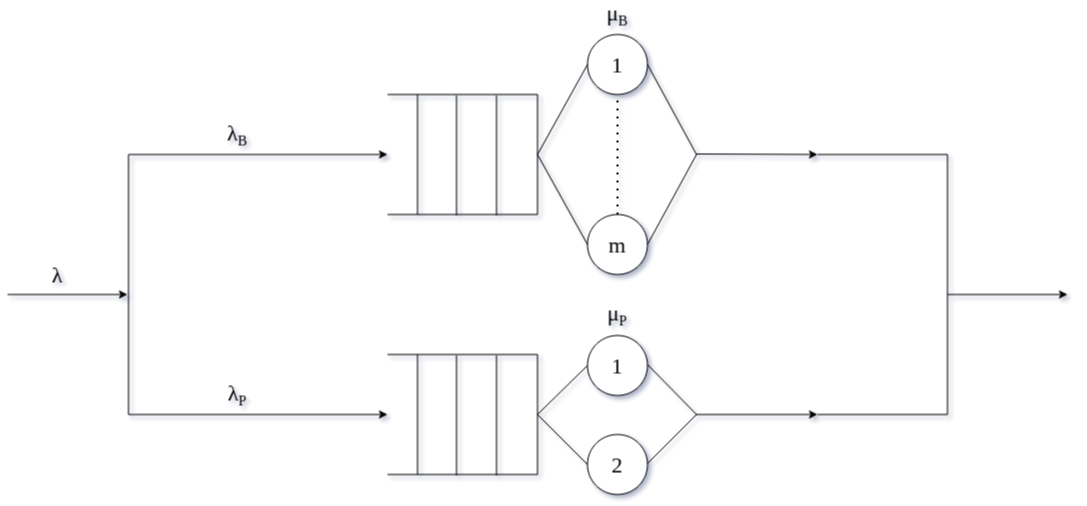
\includegraphics[width=\textwidth]{conceptual_model}
La frequenza di arrivo $\lambda$ si compone della frequenza di arrivo
$\lambda\textsubscript{B}$ e $\lambda\textsubscript{P}$, che sono rispettivamente i tassi di arrivo per richieste al bar e alla pizzeria. Una opportuna coda per ogni tipologia rappresenta la lista di attesa della tipologia stessa. Ogni servente di tipo \emph{B} rappresenta un barista assunto, che lavora con una frequenza $\mu\textsubscript{B}$. Ogni servente di tipo \emph{P}, invece, rappresenta una delle due richieste che il pizzaiolo è in grado di gestire contemporaneamente.


\subsection{Eventi del sistema e variabili di stato}
\subsection{Eventi}
\begin{center}
\begin{tabular}{ |c|c|c|c| }
	\hline
    \cellcolor{cellcolor}Indice & \cellcolor{cellcolor}Descrizione & \cellcolor{cellcolor}Attributo 1 & \cellcolor{cellcolor}Attributo 2 \\
    \hline
    \hline
    0 & Arrivo di tipo B & t & x \\
    \hline
    1 & Completamento dal server $B_1$ & t & x \\
    \hline
    .. & .. & t & x \\
    \hline
    m & Completamento dal server $B_m$ & t & x \\
    \hline
    m + 1 & Arrivo di tipo P & t & x \\
    \hline
    m + 2 & Completamento dal server $P_1$ & t & x \\
    \hline
    m + 3 & Completamento dal server $P_2$ & t & x \\
    \hline
    m + 4 & Evento di campionamento & t & x \\
    \hline
\end{tabular}
\end{center}
L'attributo \emph{t} indentifica il tempo schedulato per la successiva occorrenza
dell'evento di quel tipo; l'attributo \emph{x} identifica lo stato di attività
dell'evento.

\subsection{Variabili di stato}
\begin{itemize}
  \item $l\textsubscript{B}(t)$: numero di richieste di tipo B al centro all'istante $t$
  \item $l\textsubscript{P}(t)$: numero di richieste di tipo P al centro all'istante $t$
  \item $X\textsubscript{s}(t)$: stato del servente $s$ all'istante $t$, 
  con $s \in$ \bup, dove \bup{} è l'insieme dei serventi di tipo \textit{B} unito all'insieme dei serventi di tipo \textit{P}.
  \[
      X\textsubscript{s}(t) = 
  \begin{cases}
      1& \text{se servente s è occupato}\\ 
      0              & \text{altrimenti}
  \end{cases}
  \]	
\end{itemize}

\section{Modello delle specifiche}

\subsection{Periodo di osservazione}
Il periodo di osservazione è quello di un intero anno e ogni giorno si osserva l'intera giornata lavorativa costituita dalle due fasce orarie riportate precedentemente nelle \attach{tabelle riassuntiva dei tassi di arrivo}.

\target{interarrivi gaussiani}
\subsection{Distribuzione degli arrivi}
I valori dei vari tassi di arrivo sono stati raccolti analizzando un caso reale, anche se si tratta comunque di una stima. Per rappresentare il processo degli arrivi è stata utilizzata la distribuzione esponenziale, utilizzando $\lambda$ diversi per ogni fascia oraria. Inoltre, all'interno della singola fascia oraria, gli arrivi potrebbero essere modellati come una distribuzione gaussiana, centrata attorno all'ora in cui le richieste sono più probabili. A partire da questa osservazione, si è scelto di utilizzare la distribuzione esponenziale per modellare gli arrivi, ma la media utilizzata è pesata opportunamente per una probabilità che è tanto più alta quanto più il tempo di simulazione è vicino all'ora di massima affluenza per quella fascia oraria. Per modellare questo, si definiscono delle frequenze di interarrivo medie per ogni fascia oraria, riportate qui in minuti:
\bigskip

\begin{minipage}{.5\textwidth}
\centering             
\begin{tabular}{ |c|c|c| }
	\hline
    \cellcolor{cellcolor} Fascia oraria & \cellcolor{cellcolor}$\lambda${\textsubscript{B,W}} & \cellcolor{cellcolor}$\lambda${\textsubscript{P,W}} \\
	\hline
    \hline

	07:00 $\rightarrow$ 11:00 & 0.5 j/min & \xmark \\

    \hline
    

	11:00 $\rightarrow$ 15:00 & 0.21 j/min & \xmark \\

    \hline
    

	18:00 $\rightarrow$ 19:00 & 0.42 j/min & \xmark \\

    \hline
    

	19:00 $\rightarrow$ 23:00 & 0.21 j/min & 0.17 j/min \\

    \hline
    

	23:00 $\rightarrow$ 02:00 & 0.17 j/min & \xmark \\

    \hline
\end{tabular}
\bigskip
              
\textit{Frequenze di arrivo settimanali}
\end{minipage}
%
\begin{minipage}{.5\textwidth}
\centering
\begin{tabular}{ |c|c|c| }
	\hline
    \cellcolor{cellcolor}Fascia oraria & \cellcolor{cellcolor}$\lambda${\textsubscript{B,WE}}
    &\cellcolor{cellcolor} $\lambda${\textsubscript{P,WE}} \\
    \hline
    \hline
	07:00 $\rightarrow$ 11:00 & 0.5 j/min & \xmark \\ 
    \hline
	11:00 $\rightarrow$ 15:00 & 0.34 j/min & \xmark \\
    \hline
	18:00 $\rightarrow$ 19:00 & 0.75 j/min & \xmark \\
    \hline
	19:00 $\rightarrow$ 23:00 & 0.375 j/min & 0.5 j/min \\
    \hline
	23:00 $\rightarrow$ 02:00 & 0.34 j/min & \xmark \\
    \hline
\end{tabular}
\bigskip
              
\textit{Frequenze di arrivo fine-settimanali} 
\end{minipage} 
\bigskip

Per ogni fascia oraria si definisce una distribuzione di probabilità gaussiana:\\

\begin{minipage}{0.45\textwidth}
\begin{table}[H]
\centering
\begin{tabular}{ |c|c|c| }
	\hline
    \cellcolor{cellcolor} Fascia oraria & \cellcolor{cellcolor}$\mu$ & \cellcolor{cellcolor}$\sigma$\\
	\hline
    \hline

  	07:00 $\rightarrow$ 11:00 & 8 & 1.2 \\
    \hline	
	
	11:00 $\rightarrow$ 15:00 & 13.5 & 2 \\
    \hline
  
	18:00 $\rightarrow$ 19:00 & 18.5 & 0.4 \\  
    \hline
    
	19:00 $\rightarrow$ 23:00 & 22.5 & 2\\
    \hline
    
    23:00 $\rightarrow$ 02:00 & 24 & 0.9 \\
    \hline        
\end{tabular}
\end{table}
\end{minipage}
\hspace{0.1\textwidth}
\begin{minipage}{0.45\textwidth}
\begin{table}[H]
\centering
\begin{tabular}{ |c|c|c| }
	\hline
    \cellcolor{cellcolor} Fascia oraria & \cellcolor{cellcolor}$\mu$ & \cellcolor{cellcolor}$\sigma$\\
	\hline
    \hline
    19:00 $\rightarrow$ 23:00 & 20.5 & 1\\
    \hline
\end{tabular}
\end{table}
\end{minipage}
\bigskip

\begin{minipage}{0.45\textwidth}
\centering
\textit{Parametri delle gaussiane per richieste di tipo B}
\end{minipage}
\hspace{0.1\textwidth}
\begin{minipage}{0.45\textwidth}
\centering
\textit{Parametri delle gaussiane per richieste di tipo P}
\end{minipage}
\bigskip

La loro rappresentazione grafica è riportata \hyperlink{rappresentazione grafica gaussiane}{in fondo al documento}. 
\bigskip

Ora, supponiamo di essere all'istante di simulazione $t_0$ di un giorno settimanale, nella prima fascia oraria; in questo caso $\lambda = 0.5\ j/min$ .  Per generare il prossimo tempo di interarrivo, si usa:
\begin{center}
\key{Exponential(1/$\lambda$) * $f^n(t0)$}
\end{center}
dove $f^n(t_0)$ è il valore della distribuzione normale relativa alla fascia oraria valutata in $t_0$ e normalizzata rispetto alla fascia oraria. Nell'esempio:
\[
f^n(t_0) = \frac{f(t_0)}{F(11) - F(7)}
\]
con $F(x)$ funzione cumulativa della distribuzione gaussiana relativa alla fascia oraria 07:00 $\rightarrow$ 11:00.\\

Non si è usata una gaussiana direttamente come distribuizione del tempo di interarrivo perché avrebbe modellato una cosa diversa: in quel caso i tempi sarebbero molto più vicini al valor medio della distribuzione all'interno dell'intera fascia in esame, invece si vuole modellare che il tempo di interarrivo diminuisce in un intorno di un certo tempo. \\

La simulazione permette di disabilitare questa opzione inserendo l'opportuno \textit{flag} nel lancio del programma.


\subsection{Assunzioni}
\begin{itemize}
  \item Stato iniziale vuoto: 
  \[ 
    l\textsubscript{B}(0) + l\textsubscript{P}(0) = P(0) + B(0) = 0 
\]
  Come conseguenza, il primo evento deve essere necessariamente un arrivo e, in particolare, è un arrivo di tipo \textit{B}: la pizzeria apre alle 19.
  \item Stato finale di ogni giorno vuoto:
\[
    X\textsubscript{s}(T) = 0\ \ \ \forall s \in \mathcal{B} \cup \mathcal{P}
\]
  Con $T$ tempo di chiusura giornaliero e $\mathcal{B} \cup \mathcal{P}$ l'unione dell'insieme dei serventi di tipo \textit{B} e \textit{P}. Come conseguenza, l'ultimo evento non può essere un arrivo, e sarà quindi o una partenza o un campionamento.

  \item I tempi di servizio di ognuno dei serventi si assumono  esponenziali e indipendenti dalla fascia oraria. In particolare, ogni servente di tipo \textit{B} lavora con frequenza media pari a $\mu\textsubscript{B} = \frac{1}{2}\ j/min$; ogni servente di tipo \textit{P} lavora con frequenza media pari a $\mu\textsubscript{P} = \frac{1}{3}\ j/min$. 
  
\item l'evento di campionamento non deve seguire un evento di campionamento: non ha molto senso raccogliere due volte le statistiche se nel mezzo non è accaduto niente. Anzi: un campionamento incontrollato di questo tipo darebbe un peso maggiore al valore delle statistiche raccolte successivamente.
\end{itemize}

\subsection{Guadagni e costi}


\section{Modello analitico}
Di seguito sono rappresentate le formule utilizzate per l’analisi teorica del sistema. In particolare, tutti i centri sono stati modellati come M/M/m per i quali si hanno le seguenti formule teoriche:
\begin{minipage}{0.5\textwidth}
\begin{itemize}
\item[] \[
P(0) = \left[\sum_{i=0}^{m-1} \frac{(m\rho)^i}{i!} + \frac{(m\rho)^m}{m!(1-\rho)}\right]^{-1}
\]
\item[] \[
P_Q = \frac{(m\rho)^m}{m!(1-\rho)} \cdot p(0)
\]

\item[] \[
E(TQ) = \frac{P_Q E(S)}{1-\rho}
\]
\end{itemize}
\end{minipage}
\begin{minipage}{0.5\textwidth}
\begin{itemize}
\item[] \[
E(TS) = E(TQ) + E(S_i)
\]
\item[] \[
E(NQ)_{Erlang} = \frac{PQ \rho}{1-\rho}
\]

\item[] \[
E(NS) = E(NQ) + m\rho
\]
\end{itemize}
\end{minipage}



\section{Modello computazionale}
Il modello computazionale è stato sviluppato in \emph{Python} ed è il programma \key{simulation.py}; i parametri configurabili sono definiti invece nel file \key{configurations/Config.py}. Il programma è lanciabile da riga comando con diversi \textit{flag} che ne influenzano il comportamento, listabili con il comando: \key{python simulation.py -h} (oppure \key{python simulation.py --help}), ottenendo il seguente messaggio:
\begin{figure}[H]
\centering
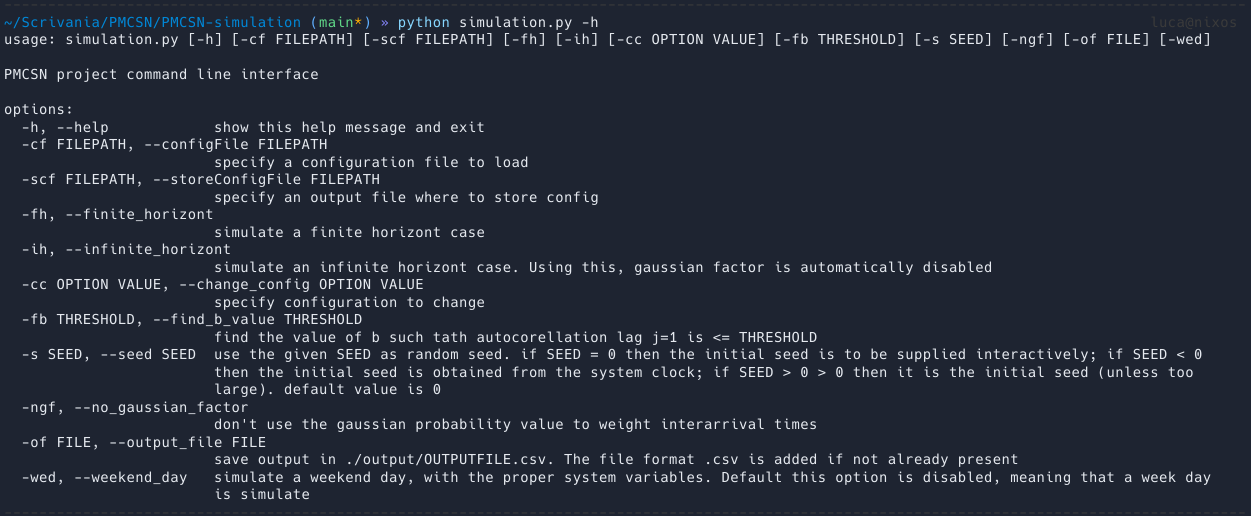
\includegraphics[width=0.8\textwidth]{program_help}
\end{figure}

In particolare, col flag \key{-cc} è possibile cambiare una qualsiasi impostazione presente nel file di configurazione specificandone il valore a riga comando, mentre col flag \key{-ngf} (cioè \key{--no_gaussian_factor}) si disabilita la normalizzazione del tempo di interarrivo col fattore gaussiano determinato secondo le modalità descritte nella \hyperlink{interarrivi gaussiani}{sezione dedicata alla distribuzione degli arrivi}. \\

Il programma è realizzato seguendo l'approccio della \textit{next-event simulation} e perciò sono state create opportune classi python, memorizzate ognuna in un file diverso. \\

Le funzioni per processare gli arrivi sono \key{processArrivalB()} e \key{processArrivalP()} al cui interno è implementatata la logica per recuperare il $\lambda$ corretto in base alla fascia oraria, il cui inverso va usato come parametro per la funzione \key{getArrivalB(m)} e \key{getArrivalP(m)} dove viene invocata la \key{Exponential(m)} dopo aver selezionato opportunamente uno \textit{stream} diverso. Le funzioni per processare le partenze sono \key{processDepartureB()}, \key{processDepartureP()}. \\

La funzione per la selezione del servente è diversa per richieste di tipo \textit{B} e \textit{P}: si tratta di \key{FindOneB()} e \key{FindOneP()}. Queste funzioni utilizzano politiche di assegnazione ai server diverse: nel primo caso la politica è di \textit{equity}, ricercando quindi il server che risulta libero da più tempo, nel secondo, invece, dovendo simulare un pizzaiolo che può infornare contemporaneamente 2 pizze, la richiesta è assegnata al primo server libero di tipo \textit{P} che si trova, scandendo la lista in ordine crescente.\\

L'evento di campionamento viene schedulato aggiungendo un valore di tempo costante generato da una chiamata a \key{Uniform(config.SAMPLING_UNIFORM_A, config.SAMPLING_UNIFORM_B)} ad il tempo minimo tra quello dei prossimi eventi schedulati:
\begin{lstlisting}[language=Python, firstnumber=242, title=\key{simulation.py}, tabsize=3,framexleftmargin={\dimexpr 1.5em+15pt}, xleftmargin={\dimexpr 1.5em+15pt},]
times = []
for index, ev in enumerate(stats.events):
	if index != e and ev.x == 1:
		times.append(ev.t)
stats.events[e].t = min(times) + samplingInterarrivalTime
\end{lstlisting}
I vari \textit{sample} che vengono raccolti durante la simulazione vengono memorizzati in una opportuna istanza di \key{SamplingList}, il cui metodo \key{append()}, oltre ad aggiungere il nuovo campione in fondo alla lista, implementa il \textit{one-pass alghoritm} secondo \textit{Welford} per ognuna delle grandezze raccolte; è quindi necessario, a fine simulazione, invocare i metodi \key{makeCorrectVariance} che divide per il numero di campioni tutte le varianze e \key{computeConfidenceInterval} per calcolare l'intervallo di confidenza per ognuna delle grandezze.

\subsection{Makefile}
Nella directory principale è presente un \key{Makefile} che aiuta ad eseguire correttamente il programma. Usando le configurazioni predisposte, nessun parametro di configurazione viene modificato: il flag \key{-cc} non viene mai usato. In particolare, il comando \key{make clean} elimina tutti i file di output \key{.csv} generati da precedenti esecuzioni. Il comando \key{make}, che corrisponde a \key{make all}, esegue, in ordine:
\begin{lstlisting}[language=Bash, numbers=none, frame=none]
rm -f ./output/*.csv
rm -f ./output/finite/*.csv
rm -f ./output/infinite/*.csv
python3 simulation.py -ih -s 123 -of week
python3 simulation.py -ih -s 123 -wed -of weekend
python3 simulation.py -fh -s 123 -of week_gauss
python3 simulation.py -fh -s 123 -of week -ngf
python3 simulation.py -fh -s 123 -of weekend_gauss -wed
python3 simulation.py -fh -s 123 -of weekend -wed -ngf
\end{lstlisting}

Questo comando è quello utilizzato per generaer gli output che verranno successivamente discussi.


\subsection{Dipendenze}
Le librerie esterne importate, di cui il programma necessita per funzionare,  sono le seguenti e sono riportate anche nel file \key{dipendenze.txt}:
\begin{itemize}
\item \key{copy}
\item \key{argparse}
\item \key{importlib}
\item \key{ast}
\item \key{math}
\item \key{scipy.stats}
\item \key{time}
\end{itemize}

\subsection{Script di supporto}


\section{Verifica}
La fase di verifica serve a capire se, rispetto al modello che io avevo, il programma implementato è corretto. Si è quindi confrontato il valore delle statistiche restituito dal simulatore con quelle teoriche e perciò si è fatto riferimento ai valori ottenuti da una esecuzione senza il peso gaussiano. I risultati ottenuti dall'esecuzione di \key{python simulation.py -s 123 -ngf [-wed]} differiscono leggermente da quelli teorici:\\

\begin{adjustbox}{width=\textwidth}
\centering
\begin{tabular}{ |c|c|c|c|c| }
\hline
\cellcolor{cellcolor} \textit{B type} & \multicolumn{2}{|c|}{\cellcolor{cellcolor}Week} & \multicolumn{2}{|c|}{\cellcolor{cellcolor}Weekend} \\
\hline
\cellcolor{cellcolor}Statistica & \cellcolor{cellcolor}Risultato teorico & \cellcolor{cellcolor}Risultato sperimentale & \cellcolor{cellcolor}Risultato teorico & \cellcolor{cellcolor}Risultato sperimentale \\
\hline
\hline
avgInterarrivals & 3.471 min & 2.984 $\pm$ 0.076 min & 2.413 min & 2.494 $\pm$ 0.025 min \\
\hline
avgWaits & 2.251 min & 2.284 $\pm$ 0.047 min & 2.524 min & 2.266 $\pm$ 0.036 min \\
\hline
avgNumNodes & 0.682 j & 0.788 $\pm$ 0.029 j & 1.102 j & 0.801 $\pm$ 0.021 j  \\
\hline
avgDelays & 0.251 min & 0.268 $\pm$ 0.014 min & 0.524 min & 0.286 $\pm$ 0.010 min \\
\hline
avgNumQueues & 0.106 j & 0.091 $\pm$ 0.008 j & 0.273 j & 0.103 $\pm$  0.005 j \\
\hline
avgService (1) & 2 min & 1.724 $\pm$ 0.047 min & 2 min & 1.772 $\pm$  0.035 min \\
\hline
avgService (2) & 2 min & 2.367 $\pm$ 0.039 min & 2 min & 2.216 $\pm$ 0.036 min \\
\hline
\end{tabular}
\end{adjustbox}
\bigskip

\begin{adjustbox}{width=\textwidth}
\centering
\begin{tabular}{ |c|c|c|c|c| }
\hline
\cellcolor{cellcolor} \textit{P type} & \multicolumn{2}{|c|}{\cellcolor{cellcolor}Week} & \multicolumn{2}{|c|}{\cellcolor{cellcolor}Weekend} \\
\hline
\cellcolor{cellcolor}Statistica & \cellcolor{cellcolor}Risultato teorico & \cellcolor{cellcolor}Risultato sperimentale & \cellcolor{cellcolor}Risultato teorico & \cellcolor{cellcolor}Risultato sperimentale \\
\hline
\hline
avgInterarrivals & 5.882 min & 4.408 $\pm$ 0.160 min & 2.000 min & 1.846 $\pm$ 0.036 min \\
\hline
avgWaits & 3.209 min & 3.465 $\pm$ 0.116 min &  6.857 min & 5.667 $\pm$ 0.151 min \\
\hline
avgNumNodes & 0.545 j & 0.761 $\pm$ 0.042 j & 3.429 j & 2.962 $\pm$ 0.046 j \\
\hline
avgDelays & 0.209 min & 0.050 $\pm$ 0.008 min & 3.857 min & 2.514 $\pm$ 0.083 min \\
\hline
avgNumQueues & 0.035 j & 0.013 $\pm$ 0.003 j & 1.929 j & 1.316 $\pm$ 0.037 j \\
\hline
avgService (1) & 3 min & 2.918 $\pm$ 0.136 min & 3 min & 2.947 $\pm$ 0.116 \\
\hline
avgService (2) & 3 min & 4.722 $\pm$ 0.201 min & 3 min & 3.361 $\pm$ 0.069 min \\
\hline

\end{tabular}
\end{adjustbox}
\bigskip

%\begin{adjustbox}{width=\textwidth}
%\centering
%\begin{tabular}{ |c|c|c|c|c|c|c| }
%\hline
%\cellcolor{cellcolor} \textit{B type} & \multicolumn{3}{|c|}{\cellcolor{cellcolor}Week} & \multicolumn{3}{|c|}{\cellcolor{cellcolor}Weekend} \\
%\hline
%\cellcolor{cellcolor}Statistica & \cellcolor{cellcolor}Risultato teorico & \cellcolor{cellcolor}Risultato sperimentale & \cellcolor{cellcolor}Errore & \cellcolor{cellcolor}Risultato teorico & \cellcolor{cellcolor}Risultato sperimentale & \cellcolor{cellcolor}Errore\\
%\hline
%\hline
%avgInterarrivals & 3.471 min & 2.984 $\pm$ 0.076 min & 0.411 & 2.413 min & 2.494 $\pm$ 0.025 min & 0.056\\
%\hline
%avgWaits & 2.251 min & 2.284 $\pm$ 0.047 min & 0 & 2.524 min & 2.266 $\pm$ 0.036 min & 0.222\\
%\hline
%avgNumNodes & 0.682 j & 0.788 $\pm$ 0.029 j & 0.0.77 & 1.102 j & 0.801 $\pm$ 0.021 j & 0.280 \\
%\hline
%avgDelays & 0.251 min & 0.268 $\pm$ 0.014 min & 0.003 & 0.524 min & 0.286 $\pm$ 0.010 min & 0.228\\
%\hline
%avgNumQueues & 0.106 j & 0.091 $\pm$ 0.008 j & 0.007 & 0.273 j & 0.103 $\pm$  0.005 j & 0.165 \\
%\hline
%avgService (1) & 2 min & 1.724 $\pm$ 0.047 min & 0.229 & 2 min & 1.772 $\pm$  0.035 min & 0.193 \\
%\hline
%avgService (2) & 2 min & 2.367 $\pm$ 0.039 min & 0.328 & 2 min & 2.216 $\pm$ 0.036 min & 0.18 \\
%\hline
%\end{tabular}
%\end{adjustbox}
%\bigskip
%
%\begin{adjustbox}{width=\textwidth}
%\centering
%\begin{tabular}{ |c|c|c|c|c|c|c| }
%\hline
%\cellcolor{cellcolor} \textit{P type} & \multicolumn{3}{|c|}{\cellcolor{cellcolor}Week} & \multicolumn{3}{|c|}{\cellcolor{cellcolor}Weekend} \\
%\hline
%\cellcolor{cellcolor}Statistica & \cellcolor{cellcolor}Risultato teorico & \cellcolor{cellcolor}Risultato sperimentale & \cellcolor{cellcolor}Errore & \cellcolor{cellcolor}Risultato teorico & \cellcolor{cellcolor}Risultato sperimentale & \cellcolor{cellcolor}Errore\\
%\hline
%\hline
%avgInterarrivals & 5.882 min & 4.408 $\pm$ 0.160 min & 1.242 & 2.000 min & 1.846 $\pm$ 0.036 min & 0.103 \\
%\hline
%avgWaits & 3.209 min & 3.465 $\pm$ 0.116 min & 0.098 & 6.857 min & 5.667 $\pm$ 0.151 min & 0.994\\
%\hline
%avgNumNodes & 0.545 j & 0.761 $\pm$ 0.042 j & 0.166 & 3.429 j & 2.962 $\pm$ 0.046 j & 0.411\\
%\hline
%avgDelays & 0.209 min & 0.050 $\pm$ 0.008 min & 0.143 & 3.857 min & 2.514 $\pm$ 0.083 min & 1.232\\
%\hline
%avgNumQueues & 0.035 j & 0.013 $\pm$ 0.003 j & 0.016 & 1.929 j & 1.316 $\pm$ 0.037 j & 0.564 \\
%\hline
%avgService (1) & 3 min & 2.918 $\pm$ 0.136 min &  & 3 min & 2.947 $\pm$ 0.116 & 0.193 \\
%\hline
%avgService (2) & 3 min & 4.722 $\pm$ 0.201 min & 0.007 & 3 min & 3.361 $\pm$ 0.069 min & 0.292 \\
%\hline
%
%\end{tabular}
%\end{adjustbox}
%\bigskip

Il motivo di tale differenza va ricercato nella bassa frequenza di arrivo: infatti, all'interno di un singolo run di tipo \textit{week}, i job processati di tipo \textit{B} non arrivano a 300, mentre quelli di tipo \textit{P} superano di poco i 50, rendendo le statistiche poco rappresentative. Perciò, si è definito un nuovo file di configurazione, 

%Inoltre, essendoci molte fasce orarie con frequenze diverse, il sistema presenta una grossa variabilità che, per essere abbattuta, necessita di un gran numero di richieste per ognuna di queste fasce. Per verificare la bontà del simulatore, si è quindi deciso di provare a cambiare delle configurazioni e analizzare i risultati ottenuti, verificando che questi tendano al risultato teorico, accettando anche un eventuale errore che non sia troppo grande. 

\subsection{\texttt{verify1.py}}
Per ovviare al problema del basso tasso di interarrivo, si è costruito il file di configurazione \key{verify1.py} che cerca di aumentare il numero di job di ogni tipologia processati nel singolo \textit{run}. Per farlo, si è definito le seguenti frequenze di interarrivo, cercando di abbattere anche il contributo di una eccessiva variabilità tra le fasce:
\begin{table}
\centering
\begin{tabular}{ |c|c|c| }
	\hline
    \cellcolor{cellcolor}Fascia oraria & \cellcolor{cellcolor}$\lambda${\textsubscript{B,W}}
    &\cellcolor{cellcolor} $\lambda${\textsubscript{P,W}} \\
    \hline
    \hline
	07:00 $\rightarrow$ 11:00 & 4.2 j/s & \xmark \\ 
    \hline
	11:00 $\rightarrow$ 15:00 & 4.2 j/s & \xmark \\
    \hline
	18:00 $\rightarrow$ 19:00 & 2.1 j/s & \xmark \\
    \hline
	19:00 $\rightarrow$ 23:00 & 2.1 j/s & 2 j/s \\
    \hline
	23:00 $\rightarrow$ 02:00 & 2.1 j/s & \xmark \\
    \hline
\end{tabular}
\end{table}

Altre configurazioni cambiate sono le seguenti:
\begin{lstlisting}[language=Python, numbers=none, title=\key{configurations/verify1.py}]
# per esprimere i tempi in secondi:
SLOTSTIME = [ (i * 3600) for i in [7, 11, 15, 18, 19, 23] ] 
STOP_B = 26 * 3600   
# per rendere il sistema stabile anche dal punto di vista analitico
MEAN_SERVICE_TIME_B = 0.5
MEAN_SERVICE_TIME_P = 0.5
# i lambda:
WEEK_LAMBDA_B = [2, 2, 0, 3, 3, 3]
WEEK_LAMBDA_P = 1.7
\end{lstlisting}

Eseguendo il comando \key{python simulation.py -s 123 -ngf -cf configurations/verify1.py}, si ottengono i seguenti risultati:

%        statistic          mean    variance      conf int
%  avg interarrivals .. :  0.466     0.002         0.000
%  avg wait ........... :  0.337     0.000         0.000
%  avg # in node ...... :  0.730     0.008         0.001
%  avg delay .......... :  0.037     0.000         0.000
%  avg # in queue ..... :  0.083     0.001         0.000

\begin{table}[H]
\centering
\begin{tabular}{ |c|c|c| }
\hline
\cellcolor{cellcolor} \textit{B type} & \multicolumn{2}{|c|}{\cellcolor{cellcolor}Week} \\
\hline
\cellcolor{cellcolor}Statistica & \cellcolor{cellcolor}Risultato teorico & \cellcolor{cellcolor}Risultato sperimentale \\
\hline
\hline
avgInterarrivals & 0.317 s & 0.466 $\pm$ 0.002 s \\
\hline
avgWaits & 0.415 s & 0.337 $\pm$ 0.000 s \\
\hline
avgNumNodes & 1.394 j & 0.739 $\pm$ 0.008 j \\
\hline
avgDelays & 0.115 s & 0.037 $\pm$ 0.000 s \\
\hline
avgNumQueues & 0.449 j & 0.083 $\pm$ 0.000 j \\
\hline
avgService (1) & 0.3 s & 0.300 $\pm$ 0.000 s \\
\hline
avgService (2) & 0.3 s & 0.300 $\pm$ 0.000 s \\
\hline
\end{tabular}
\end{table}
\bigskip

\begin{table}[H]
\centering
\begin{tabular}{ |c|c|c| }
\hline
\cellcolor{cellcolor} \textit{P type} & \multicolumn{2}{|c|}{\cellcolor{cellcolor}Week} \\
\hline
\cellcolor{cellcolor}Statistica & \cellcolor{cellcolor}Risultato teorico & \cellcolor{cellcolor}Risultato sperimentale \\
\hline
\hline
avgInterarrivals & 0.588 s & 0.593 $\pm$ 0.000 s \\
\hline
avgWaits & 0.610 s & 0.603 $\pm$ 0.000 s \\
\hline
avgNumNodes & 1.037 j & 1.017 $\pm$ 0.001 j \\
\hline
avgDelays & 0.110 s & 0.105 $\pm$ 0.000 s \\
\hline
avgNumQueues & 0.187 j & 0.176 $\pm$ 0.000 j \\
\hline
avgService (1) & 0.5 s & 0.496 $\pm$ 0.000 s \\
\hline
avgService (2) & 0.5 s & 0.501 $\pm$ 0.000 s \\
\hline
\end{tabular}
\end{table}
\bigskip

Si può osservare come i valori teorici per le richieste di tipo \textit{P}, che sono state in tutto 24407, cominciano a convergere ai valori teorici. Per le richieste di tipo \textit{B}, nonostante siano state 181785, i valori ottenuti sono ancora lontani da quelli teorici.\\

Si può però osservare che la frequenza di interarrivo media nella prima metà della giornata è più piccola, e perciò il numero di job processati e di campioni fatti nelle prime 8 ore sarà minore rispetto a quelli fatti nelle seconde 8. Per questo motivo, nel calcolo della media globale, i dati delle statistiche raccolti nella prima metà della giornata tende a pesare di meno rispetto a quelli raccolti nella seconda metà. Alla luce di questo comportamento, è stata aggiunta una nuova opzione, attiva per default, che serve a \textit{spezzare} l'analisi media nelle due fasce orarie. In particolare, si raccolgono i dati in entrambe le metà separatamente, calcolando per ogni statistica la sua media e varianza per poi mediarle col numero di job processati:
\[
	\mu_{glob} = \frac{n_1 \mu_i + n_2 \mu_2}{n_1 + n_2}
\]
Dove $n_1$ ed $n_2$ sono rispettivamente il numero di job processati nella prima e nella seconda metà, mentre $\mu_1$ e $\mu_2$ sono le medie raccolte nelle due metà. Per disabilitare questa funzione, bisogna specificare a riga comando il flag \key{-ns}. \\

I risultati ottenuti dal comando \key{python simulation.py -s 123 -ngf -cf configurations/verify1.py} senza aver cambiato nulla nel file di configurazione rispetto al caso precedente sono i seguenti:

\begin{table}[H]
\centering
\begin{tabular}{ |c|c|c| }
\hline
\cellcolor{cellcolor} \textit{B type} & \multicolumn{2}{|c|}{\cellcolor{cellcolor}Week} \\
\hline
\cellcolor{cellcolor}Statistica & \cellcolor{cellcolor}Risultato teorico & \cellcolor{cellcolor}Risultato sperimentale \\
\hline
\hline
avgInterarrivals & 0.400 s & 0.399 $\pm$ 0.000 s \\
\hline
avgWaits & 0.353 s & 0.355 $\pm$ 0.000 s \\
\hline
avgNumNodes & 0.894 j & 0.938 $\pm$ 0.000 j \\
\hline
avgDelays & 0.053 s & 0.055 $\pm$ 0.000 s \\
\hline
avgNumQueues & 0.144 j & 0.156 $\pm$ 0.000 j \\
\hline
avgService (1) & 0.3 s & 0.300 $\pm$ 0.000 s \\
\hline
avgService (2) & 0.3 s & 0.299 $\pm$ 0.000 s \\
\hline
\end{tabular}
\end{table}
\bigskip

Alla luce degli esperimenti fatti, si può concludere che il simulatore risponde bene ai cambiamenti di configurazione e che, con un numero adeguato di job, produce risultati fedeli a quelli teorici dimostrando così di essere fedele al modello di sistema in esame. 


\section{Validazione}
Nella fase di validazione il quesito fondamentale è: "Stiamo costruendo il prodotto giusto?" Tuttavia, durante il processo di validazione, si sono riscontrate delle sfide significative nell'utilizzo dell'analisi a orizzonte finito, principalmente dovute al numero limitato di job processati. Un aspetto critico che ha reso l'analisi a orizzonte finito inadeguata è il basso numero di job processati in ciascun \textit{run} di simulazione, una caratteristica intrinseca del caso di studio in esame. Questa limitazione ha comportato un campione statistico ridotto e, di conseguenza, una maggiore variabilità nei risultati osservati. In altre parole, la variabilità è emersa come una problematica principale a causa della limitata quantità di dati disponibili. \\

È importante notare che, in un contesto in cui avessimo processato un numero significativamente maggiore di job in ogni run, la variabilità non avrebbe avuto un impatto significativo. \\

Per affrontare questa sfida, si è deciso di adottare un'analisi a orizzonte infinito in modo da ottenere risultati più stabili. In questa fase di validazione, verifichiamo se, per ciascuna fascia oraria, le statistiche generate dal nostro simulatore convergono ai valori teorici, considerati come punti di riferimento per il nostro sistema. Questo approccio ci assicura che il sistema software risponda alle caratteristiche previste e ai requisiti desiderati. 

\subsection{Analisi a orizzonte infinito}
%Per svolgere l'analisi a orizzonte infinito si può utilizzare il comando \key{make infinite-week} e \key{make infinite-weekend}, che eseguono rispettivamente: \key{python3 simulation.py -ih -s 123 -of week} e \key{python3 simulation.py -ih -s 123 -wed -of weekend}; è opportuno eliminare eventuali file di output csv già presenti. Per questo tipo di analisi, è possibile specificare il flag \key{-fb THRESHOLD} con cui si determina dinamicamente il numero di campioni da fare per il singolo batch. Il valore scelto è quello che rende il valore di autocorrelazione minore di \key{THRESHOLD} per \textit{lag j} $= 1$, per ogni statistica. Utilizzando $k = 128$ \textit{batches}, ognuno di $b = 1024$ campioni, si ottiene che il valore di autocorrelazione per \textit{lag j} $= 1 < 0.2$. L'analisi è stata fatta per ogni tipo di richiesta, per ogni statistica e per ogni fascia oraria, sia nel caso di giorno settimanale che di giorno fine-settimanale. I risultati vengono riportati in forma tabellare e in forma grafica, utilizzando nelle tabelle il risultato sperimentale relativo all'ultimo \textit{batch}:\\

Per condurre un'analisi a orizzonte infinito, è necessario utilizzare i seguenti comandi:

\begin{itemize}
  \item \key{make infinite-week}: esegue \key{python3 simulation.py -ih -s 123 -of week}. Effettua l'analisi per il giorno lavorativo della settimana.
  \item \key{make infinite-weekend}: esegue \texttt{python3 simulation.py -ih -s 123 -wed -of weekend}. Effettua l'analisi per il fine settimana.
\end{itemize}

È fondamentale notare che, prima di eseguire questi comandi, è consigliabile eliminare eventuali file di output CSV già presenti al fine di evitare confusione nei risultati.\\

Per determinare i parametri dell'analisi, è possibile specificare il flag \key{-fb THRESHOLD}, il quale consente di determinare dinamicamente il numero di campioni da raccogliere per ogni batch. Il parametro \key{THRESHOLD} specifica che il valore di autocorrelazione per lag \key{j = 1} di ogni statistica non deve superare quel valore. Utilizzando \key{k = 128} batches, ciascuno con \key{b = 1024} campioni, l'autocorrelazione per lag \texttt{j = 1} è inferiore a \key{0.2}, contribuendo così alla stabilità e all'affidabilità dei risultati.\\

L'analisi viene condotta per ciascun tipo di richiesta e per ciascuna statistica di interesse, coprendo tutte le fasce orarie sia nei giorni lavorativi che nei giorni del fine settimana. I risultati vengono presentati in forma tabellare e grafica; in particolare, nelle tabelle si riportano i risultati sperimentali ottenuti mediando su tutti i batch con un intervallo di confidenza al 95\%.\\


\begin{adjustbox}{width=\textwidth}
\centering
\begin{tabular}{ |c|c|c|c|c|c|c|c| }
\cline{2-7}
\multicolumn{1}{c}{} & \multicolumn{6}{|c|}{\cellcolor{cellcolor}\textit{B type - Interarrivals}}\\
\cline{2-7}
\multicolumn{1}{c|}{} & \cellcolor{cellcolor}Slot & \cellcolor{cellcolor}Risultato teorico & \cellcolor{cellcolor}Risultato sperimentale &  \cellcolor{cellcolor}Media nell'intervallo &
\cellcolor{cellcolor}Errore & \cellcolor{cellcolor}Link all'immagine\\
\cline{2-7}
\noalign{\vspace{0.5ex}}
\hline
\cellcolor{cellcolor}& 0 & 2.000 min & 2.000 $\pm$ 0.014 min & \checkmark & & \hyperlink{interarrivo infinito week slot 0}{link}  \\ 
\cline{2-7}
\cellcolor{cellcolor}& 1 & 4.762 min & 4.950 $\pm$ 0.389 min & \checkmark & & \hyperlink{interarrivo infinito week slot 1}{link}\\
\cline{2-7}
\cellcolor{cellcolor}& 3 & 2.381 min & 2.614 $\pm$ 0.477 min & \checkmark & & \hyperlink{interarrivo infinito week slot 3}{link}\\
\cline{2-7}
\cellcolor{cellcolor}& 4 & 4.762 min & 5.154 $\pm$ 0.811 min & \checkmark & & \hyperlink{interarrivo infinito week slot 4}{link}\\
\cline{2-7}
\multirow{-6}{*}{\rotatebox[origin=c]{90}{\cellcolor{cellcolor}Week}} & 5 & 5.882 min & 6.217 $\pm$ 0.074 min & \checkmark & & \hyperlink{interarrivo infinito week slot 5}{link}\\
\hline
\hline
\cellcolor{cellcolor}& 0 & 2.000 min & 2.000 $\pm$ 0.014 min & \checkmark & & \hyperlink{interarrivo infinito weekend slot 0}{link}\\ 
\cline{2-7}
\cellcolor{cellcolor}& 1 & 2.941 min & 3.091 $\pm$ 0.322 min & \checkmark & &\hyperlink{interarrivo infinito weekend slot 1}{link}\\
\cline{2-7}
\cellcolor{cellcolor}& 3 & 1.333 min & 1.460 $\pm$ 0.259 min & \checkmark & & \hyperlink{interarrivo infinito weekend slot 3}{link}\\
\cline{2-7}
\cellcolor{cellcolor}& 4 & 2.667 min & 2.794 $\pm$ 0.268 min & \checkmark & & \hyperlink{interarrivo infinito weekend slot 4}{link}\\
\cline{2-7}
\multirow{-6}{*}{\rotatebox[origin=c]{90}{\cellcolor{cellcolor}Weekend}} & 5 & 2.941 min & 3.065 $\pm$ 0.285 min & \checkmark & & \hyperlink{interarrivo infinito weekend slot 5}{link}\\
\hline
\end{tabular}
\end{adjustbox}
\bigskip

\begin{adjustbox}{width=\textwidth}
\centering
\begin{tabular}{ |c|c|c|c|c|c|c|c|c| }
\cline{2-8}
\multicolumn{1}{c}{} & \multicolumn{7}{|c|}{\cellcolor{cellcolor}\textit{B type - Waits}}\\
\cline{2-8}
\multicolumn{1}{c|}{} & \cellcolor{cellcolor}Slot & \cellcolor{cellcolor}Risultato teorico & \cellcolor{cellcolor}Risultato sperimentale &  \cellcolor{cellcolor}Media nell'intervallo &
\cellcolor{cellcolor}Errore & \cellcolor{cellcolor}Link all'immagine & \cellcolor{cellcolor} Rispetta \textit{QoS}\\
\cline{2-8}
\noalign{\vspace{0.5ex}}
\hline
\cellcolor{cellcolor}& 0 & 2.667 min & 2.665 $\pm$ 0.035 min & \checkmark & & \hyperlink{attesa infinita week slot 0}{link} & \checkmark \\ 
\cline{2-8}
\cellcolor{cellcolor}& 1 & 2.092 min & 2.083 $\pm$ 0.018 min & \checkmark & & \hyperlink{attesa infinita week slot 1}{link}& \checkmark \\ 
\cline{2-8}
\cellcolor{cellcolor}& 3 & 2.428 min & 2.440 $\pm$ 0.027 min & \checkmark & & \hyperlink{attesa infinita week slot 3}{link}& \checkmark \\ 
\cline{2-8}
\cellcolor{cellcolor}& 4 & 2.092 min & 2.086 $\pm$ 0.021 min & \checkmark & & \hyperlink{attesa infinita week slot 4}{link}& \checkmark \\ 
\cline{2-8}
\multirow{-6}{*}{\rotatebox[origin=c]{90}{\cellcolor{cellcolor}Week}} & 5 & 2.060 min & 2.067 $\pm$ 0.023 min & \checkmark & & \hyperlink{attesa infinita week slot 5}{link}&  \checkmark \\ 
\hline
\hline
\cellcolor{cellcolor}& 0 & 2.667 min & 2.665 $\pm$ 0.035 min & \checkmark & & \hyperlink{attesa infinita weekend slot 0}{link}& \checkmark \\ 
\cline{2-8}
\cellcolor{cellcolor}& 1 & 2.261 min & 2.257 $\pm$ 0.024 min & \checkmark & &\hyperlink{attesa infinita weekend slot 1}{link}& \checkmark \\ 
\cline{2-8}
\cellcolor{cellcolor}& 3 & 4.571 min & 4.499 $\pm$ 0.115 min & \checkmark & & \hyperlink{attesa infinita weekend slot 3}{link}& \xmark \\ 
\cline{2-8}
\cellcolor{cellcolor}& 4 & 2.327 min & 2.339 $\pm$ 0.031 min & \checkmark & & \hyperlink{attesa infinita weekend slot 4}{link}& \checkmark \\ 
\cline{2-8}
\multirow{-6}{*}{\rotatebox[origin=c]{90}{\cellcolor{cellcolor}Weekend}} & 5 & 2.261 min & 2.246 $\pm$ 0.025 min & \checkmark & & \hyperlink{attesa infinita weekend slot 5}{link}& \checkmark \\ 
\hline
\end{tabular}
\end{adjustbox}
\bigskip

\begin{adjustbox}{width=\textwidth}
\centering
\begin{tabular}{ |c|c|c|c|c|c|c|c| }
\cline{2-7}
\multicolumn{1}{c}{} & \multicolumn{6}{|c|}{\cellcolor{cellcolor}\textit{B type - Num. in the nodes}}\\
\cline{2-7}
\multicolumn{1}{c|}{} & \cellcolor{cellcolor}Slot & \cellcolor{cellcolor}Risultato teorico & \cellcolor{cellcolor}Risultato sperimentale &  \cellcolor{cellcolor}Media nell'intervallo &
\cellcolor{cellcolor}Errore & \cellcolor{cellcolor}Link all'immagine\\
\cline{2-7}
\noalign{\vspace{0.5ex}}
\hline
\cellcolor{cellcolor}& 0 & 1.333 min & 1.336 $\pm$ 0.021 min & \checkmark & & \hyperlink{centro infinito week slot 0}{link}  \\ 
\cline{2-7}
\cellcolor{cellcolor}& 1 & 0.439 min & 0.440 $\pm$ 0.006 min & \checkmark & & \hyperlink{centro infinito week slot 1}{link}\\
\cline{2-7}
\cellcolor{cellcolor}& 3 & 1.020 min & 1.031 $\pm$ 0.016 min & \checkmark & & \hyperlink{centro infinito week slot 3}{link}\\
\cline{2-7}
\cellcolor{cellcolor}& 4 & 0.439 min & 0.440 $\pm$ 0.007 min & \checkmark & & \hyperlink{centro infinito week slot 4}{link}\\
\cline{2-7}
\multirow{-6}{*}{\rotatebox[origin=c]{90}{\cellcolor{cellcolor}Week}} & 5 & 0.350 min & 0.355 $\pm$ 0.005 min & \checkmark & & \hyperlink{centro infinito week slot 5}{link}\\
\hline
\hline
\cellcolor{cellcolor}& 0 & 1.333 min & 1.336 $\pm$ 0.021 min & \checkmark & & \hyperlink{centro infinito weekend slot 0}{link}\\ 
\cline{2-7}
\cellcolor{cellcolor}& 1 & 0.769 min & 0.773 $\pm$ 0.011 min & \checkmark & &\hyperlink{centro infinito weekend slot 1}{link}\\
\cline{2-7}
\cellcolor{cellcolor}& 3 & 3.429 min & 3.399 $\pm$ 0.095 min & \checkmark & & \hyperlink{centro infinito weekend slot 3}{link}\\
\cline{2-7}
\cellcolor{cellcolor}& 4 & 0.873 min & 0.881 $\pm$ 0.014 min & \checkmark & & \hyperlink{centro infinito weekend slot 4}{link}\\
\cline{2-7}
\multirow{-6}{*}{\rotatebox[origin=c]{90}{\cellcolor{cellcolor}Weekend}} & 5 & 0.769 min & 0.769 $\pm$ 0.011 min & \checkmark & & \hyperlink{centro infinito weekend slot 5}{link}\\
\hline
\end{tabular}
\end{adjustbox}
\bigskip

\begin{adjustbox}{width=\textwidth}
\centering
\begin{tabular}{ |c|c|c|c|c|c|c|c| }
\cline{2-7}
\multicolumn{1}{c}{} & \multicolumn{6}{|c|}{\cellcolor{cellcolor}\textit{B type - Delays}}\\
\cline{2-7}
\multicolumn{1}{c|}{} & \cellcolor{cellcolor}Slot & \cellcolor{cellcolor}Risultato teorico & \cellcolor{cellcolor}Risultato sperimentale &  \cellcolor{cellcolor}Media nell'intervallo &
\cellcolor{cellcolor}Errore & \cellcolor{cellcolor}Link all'immagine\\
\cline{2-7}
\noalign{\vspace{0.5ex}}
\hline
\cellcolor{cellcolor}& 0 & 0.667 min & 0.671 $\pm$ 0.027 min & \checkmark & & \hyperlink{ritardo infinito week slot 0}{link}  \\ 
\cline{2-7}
\cellcolor{cellcolor}& 1 & 0.092 min & 0.100 $\pm$ 0.006 min & \xmark & 0.002 & \hyperlink{ritardo infinito week slot 1}{link}\\
\cline{2-7}
\cellcolor{cellcolor}& 3 & 0.428 min & 0.455 $\pm$ 0.019 min & \xmark & 0.008 & \hyperlink{ritardo infinito week slot 3}{link}\\
\cline{2-7}
\cellcolor{cellcolor}& 4 & 0.092 min & 0.098 $\pm$ 0.007 min & \checkmark & & \hyperlink{ritardo infinito week slot 4}{link}\\
\cline{2-7}
\multirow{-6}{*}{\rotatebox[origin=c]{90}{\cellcolor{cellcolor}Week}} & 5 & 0.060 min & 0.072 $\pm$ 0.007 min & \xmark & 0.005 & \hyperlink{ritardo infinito week slot 5}{link}\\
\hline
\hline
\cellcolor{cellcolor}& 0 & 0.667 min & 0.671 $\pm$ 0.027 min & \checkmark & & \hyperlink{ritardo infinito weekend slot 0}{link}\\ 
\cline{2-7}
\cellcolor{cellcolor}& 1 & 0.261 min & 0.268 $\pm$ 0.014 min & \checkmark & &\hyperlink{ritardo infinito weekend slot 1}{link}\\
\cline{2-7}
\cellcolor{cellcolor}& 3 & 2.571 min & 2.519 $\pm$ 0.108 min & \checkmark & & \hyperlink{ritardo infinito weekend slot 3}{link}\\
\cline{2-7}
\cellcolor{cellcolor}& 4 & 0.327 min & 0.342 $\pm$ 0.020 min & \checkmark &  & \hyperlink{ritardo infinito weekend slot 4}{link}\\
\cline{2-7}
\multirow{-6}{*}{\rotatebox[origin=c]{90}{\cellcolor{cellcolor}Weekend}} & 5 & 0.261 min & 0.265 $\pm$ 0.014 min & \checkmark & & \hyperlink{ritardo infinito weekend slot 5}{link}\\
\hline
\end{tabular}
\end{adjustbox}
\bigskip

\begin{adjustbox}{width=\textwidth}
\centering
\begin{tabular}{ |c|c|c|c|c|c|c|c| }
\cline{2-7}
\multicolumn{1}{c}{} & \multicolumn{6}{|c|}{\cellcolor{cellcolor}\textit{B type - Num. in the queue}}\\
\cline{2-7}
\multicolumn{1}{c|}{} & \cellcolor{cellcolor}Slot & \cellcolor{cellcolor}Risultato teorico & \cellcolor{cellcolor}Risultato sperimentale &  \cellcolor{cellcolor}Media nell'intervallo &
\cellcolor{cellcolor}Errore & \cellcolor{cellcolor}Link all'immagine\\
\cline{2-7}
\noalign{\vspace{0.5ex}}
\hline
\cellcolor{cellcolor}& 0 & 0.333 min & 0.339 $\pm$ 0.015 min & \checkmark & & \hyperlink{coda infinita week slot 0}{link}  \\ 
\cline{2-7}
\cellcolor{cellcolor}& 1 & 0.019 min & 0.021 $\pm$ 0.001 min & \xmark & 0.001 & \hyperlink{coda infinita week slot 1}{link}\\
\cline{2-7}
\cellcolor{cellcolor}& 3 & 0.180 min & 0.194 $\pm$ 0.005 min & \xmark &0.009  & \hyperlink{coda infinita week slot 3}{link}\\
\cline{2-7}
\cellcolor{cellcolor}& 4 & 0.019 min & 0.021 $\pm$ 0.001 min & \xmark & 0.001 & \hyperlink{coda infinita week slot 4}{link}\\
\cline{2-7}
\multirow{-6}{*}{\rotatebox[origin=c]{90}{\cellcolor{cellcolor}Week}} & 5 & 0.010 min & 0.013 $\pm$ 0.001 min & \xmark & 0.002 & \hyperlink{coda infinita week slot 5}{link}\\
\hline
\hline
\cellcolor{cellcolor}& 0 & 0.333 min & 0.339 $\pm$ 0.015 min & \checkmark & & \hyperlink{coda infinita weekend slot 0}{link}\\ 
\cline{2-7}
\cellcolor{cellcolor}& 1 & 0.089 min & 0.093 $\pm$ 0.005 min & \checkmark & &\hyperlink{coda infinita weekend slot 1}{link}\\
\cline{2-7}
\cellcolor{cellcolor}& 3 & 1.929 min & 1.910 $\pm$ 0.087 min & \checkmark & & \hyperlink{coda infinita weekend slot 3}{link}\\
\cline{2-7}
\cellcolor{cellcolor}& 4 & 0.123 min & 0.130 $\pm$ 0.008 min & \checkmark &  & \hyperlink{coda infinita weekend slot 4}{link}\\
\cline{2-7}
\multirow{-6}{*}{\rotatebox[origin=c]{90}{\cellcolor{cellcolor}Weekend}} & 5 & 0.089 min & 0.092 $\pm$ 0.005 min & \checkmark & & \hyperlink{coda infinita weekend slot 5}{link}\\
\hline
\end{tabular}
\end{adjustbox}
\bigskip

\begin{adjustbox}{width=\textwidth}
\centering
\begin{tabular}{ |c|c|c|c|c|c|c|c|c| }
\cline{2-8}
\multicolumn{1}{c}{} & \multicolumn{7}{|c|}{\cellcolor{cellcolor}\textit{P type - all statistics in the slot}}\\
\cline{2-8}
\multicolumn{1}{c|}{} & \cellcolor{cellcolor}Statistica & \cellcolor{cellcolor}Risultato teorico & \cellcolor{cellcolor}Risultato sperimentale &  \cellcolor{cellcolor}Media nell'intervallo &
\cellcolor{cellcolor}Errore & \cellcolor{cellcolor}Link all'immagine & \cellcolor{cellcolor} Rispetta QoS\\
\cline{2-8}
\noalign{\vspace{0.5ex}}
\cline{1-7}
\cellcolor{cellcolor}& Interarrivo & 5.882 min & 6.145 $\pm$ 0.499 min & \checkmark & & \hyperlink{interarrivo infinito week P}{link} & \multicolumn{1}{c}{} \\ 
\cline{2-8} 
\cellcolor{cellcolor}& Attesa & 3.209 min & 3.223 $\pm$ 0.038 min & \checkmark & & \hyperlink{attesa infinita week P}{link} & \checkmark \\
\cline{2-8}
\cellcolor{cellcolor}& Num. nel nodo & 0.545 min & 0.548 $\pm$ 0.009 min & \checkmark & & \hyperlink{centro infinito week P}{link} & \multicolumn{1}{c}{}\\
\cline{2-7}
\cellcolor{cellcolor}& Ritardo & 0.209 min & 0.229 $\pm$ 0.017 min & \xmark & 0.003 & \hyperlink{ritardo infinito week P}{link} & \multicolumn{1}{c}{}\\
\cline{2-7}
\multirow{-6}{*}{\rotatebox[origin=c]{90}{\cellcolor{cellcolor}Week}} & Num. in coda & 0.035 min & 0.040 $\pm$ 0.003 min & \xmark & 0.002	 & \hyperlink{coda infinita week P}{link} & \multicolumn{1}{c}{}\\
\cline{1-7}
\noalign{\vspace{0.5ex}}
\cline{1-7}
\cellcolor{cellcolor}& Interarrivo & 2.000 min & 2.114 $\pm$ 0.228 min & \checkmark & & \hyperlink{interarrivo infinito weekend P}{link} & \multicolumn{1}{c}{} \\ 
\cline{2-8}
\cellcolor{cellcolor}& Attesa & 6.867 min & 6.979 $\pm$ 0.281 min & \checkmark & & \hyperlink{attesa infinita weekend P}{link} & \checkmark \\
\cline{2-8}
\cellcolor{cellcolor}& Num. nel nodo & 3.429 min & 3.505 $\pm$ 0.150 min & \checkmark & & \hyperlink{centro infinito weekend P}{link} & \multicolumn{1}{c}{}\\
\cline{2-7}
\cellcolor{cellcolor}& Ritardo & 3.857 min & 3.985 $\pm$ 0.267 min & \checkmark & & \hyperlink{ritardo infinito weekend P}{link} & \multicolumn{1}{c}{}\\
\cline{2-7}
\multirow{-6}{*}{\rotatebox[origin=c]{90}{\cellcolor{cellcolor}Weekend}} & Num. in coda & 1.929 min & 2.010 $\pm$ 0.139 min & \checkmark & & \hyperlink{coda infinita weekend P}{link} & \multicolumn{1}{c}{}\\
\cline{1-7}
\end{tabular}
\end{adjustbox}
\bigskip

L'analisi a orizzonte infinito ha dimostrato che la maggior parte dei risultati converge in modo affidabile ai valori teorici previsti per il caso di studio in esame, confermando così l'accuratezza del nostro simulatore nel rappresentare il comportamento del sistema in uno stato stazionario. Tuttavia, un aspetto interessante emerge quando ripetiamo l'analisi utilizzando un seme iniziale diverso, specificamente il seme \key{12345}, con il comando \key{make clean infinite-weekend SEED=12345}. In questo caso, notiamo che la maggior parte degli errori viene azzerata, e gli altri risultano notevolmente ridotti. Questo suggerisce che il caso con il seme iniziale pari a \key{123} potrebbe essere considerato come un caso particolarmente sfortunato per l'analisi delle statistiche.\\

È interessante notare anche che nei casi in cui la frequenza di arrivo è leggermente più alta, come nel fine settimana, questi errori risultano azzerati anche con lo stesso seme \key{123}. Ciò evidenzia come la bassa frequenza di arrivo possa influenzare la precisione delle stime di queste grandezze, persino nell'analisi a orizzonte infinito. 

\section{Analisi dei costi e dei guadagni}
Per effettuare l'analisi dei costi e dei guadagni sul caso di studio in esame è stata eseguita un'analisi a orizzonte finito che, seppur poco rappresentativa in ambito di validazione, è quella che permette effettivamente di valutare le entrate e le uscite per un sistema con queste specifiche. 

\subsection{Analisi a orizzonte finito}
Con questo metodo, il sistema viene simulato per una durata pari a 16 ore lavorative effettive, prendendo in considerazione la variazione dei tassi di arrivo durante il passaggio da una fascia oraria all'altra. Per garantire la validità dell'analisi a orizzonte infinito, è essenziale che lo stato iniziale e lo stato finale del sistema siano identici. Si iniza ogni simulazione con il sistema in uno stato vuoto e ci si assicura che, al termine di ogni simulazione, il sistema sia nuovamente nello stato vuoto.\\

Simuliamo la giornata lavorativa per 1024 volte e, in ogni esecuzione, partiamo da uno stato vuoto, reimpostiamo tutte le statistiche e continuiamo senza alterare lo stato del generatore dei numeri casuali. Questo approccio garantisce l'indipendenza tra le diverse esecuzioni e ci consente di ottenere risultati affidabili per l'analisi a orizzonte infinito.\\

Anche qui l'analisi viene condotta per ciascun tipo di richiesta limitandoci però ai soli tempi di risposta, sia introducendo il fattore gaussiano che non. I risultati vengono presentati in forma tabellare e grafica; in particolare, nelle tabelle si riportano i risultati sperimentali ottenuti mediando su tutti i \textit{run} con un intervallo di confidenza al 95\%.\\


\begin{adjustbox}{width=\textwidth}
\centering
\begin{tabular}{ |c|c|c|c|c|c|c|c|c| }
\cline{2-8}
\multicolumn{1}{c}{} & \multicolumn{7}{|c|}{\cellcolor{cellcolor}\textit{Analisi senza fattore gaussiano}}\\
\cline{2-8}
\multicolumn{1}{c|}{} & \cellcolor{cellcolor}Statistica & \cellcolor{cellcolor}Risultato teorico & \cellcolor{cellcolor}Risultato sperimentale &  \cellcolor{cellcolor}Media nell'intervallo &
\cellcolor{cellcolor}Errore & \cellcolor{cellcolor}Link all'immagine & \cellcolor{cellcolor} Rispetta QoS\\
\cline{2-8}
\noalign{\vspace{0.5ex}}
\cline{1-8}
\cellcolor{cellcolor}& \makecell{Attesa di\\ tipo B} & 2.251 min & 2.455 $\pm$ 0.023 min & \xmark & 0.181 & \hyperlink{attesa finita week B no gau}{link} & \checkmark \\ 
\cline{2-8}
\multirow{-3}{*}{\rotatebox[origin=c]{90}{\cellcolor{cellcolor}Week}} & \makecell{Attesa di\\ tipo P} & 3.209 min & 3.212 $\pm$ 0.049 min & \checkmark & & \hyperlink{attesa finita week P no gau}{link} & \checkmark \\

\cline{1-8}
\noalign{\vspace{0.5ex}}
\cline{1-8}

\cellcolor{cellcolor}&\makecell{Attesa di\\ tipo B} & 2.524 min & 2.761 $\pm$ 0.032 min & \xmark & 0.205	 & \hyperlink{attesa finita weekend B no gau}{link} & \checkmark \\
\cline{2-8}
\multirow{-3}{*}{\rotatebox[origin=c]{90}{\cellcolor{cellcolor}Weekend}} & \makecell{Attesa di\\ tipo P} & 6.857 min & 5.813 $\pm$ 0.150 min & \xmark & 0.894 & \hyperlink{attesa finita weekend P no gau}{link} & \checkmark\\
\cline{1-8}

\end{tabular}
\end{adjustbox}
\bigskip

\begin{adjustbox}{width=\textwidth}
\centering
\begin{tabular}{ |c|c|c|c|c|c|c|c|c| }
\cline{2-8}
\multicolumn{1}{c}{} & \multicolumn{7}{|c|}{\cellcolor{cellcolor}\textit{Analisi con fattore gaussiano}}\\
\cline{2-8}
\multicolumn{1}{c|}{} & \cellcolor{cellcolor}Statistica & \cellcolor{cellcolor}Risultato teorico & \cellcolor{cellcolor}Risultato sperimentale &  \cellcolor{cellcolor}Media nell'intervallo &
\cellcolor{cellcolor}Errore & \cellcolor{cellcolor}Link all'immagine & \cellcolor{cellcolor} Rispetta QoS\\
\cline{2-8}
\noalign{\vspace{0.5ex}}
\cline{1-8}
\cellcolor{cellcolor}& \makecell{Attesa di\\ tipo B} & 2.251 min & 2.184 $\pm$ 0.027 min & \xmark & 0.040 & \hyperlink{attesa finita week B gau}{link} & \checkmark \\ 
\cline{2-8}
\multirow{-3}{*}{\rotatebox[origin=c]{90}{\cellcolor{cellcolor}Week}} & \makecell{Attesa di\\ tipo P} & 3.209 min & 3.082 $\pm$ 0.078 min & \xmark & 0.049 & \hyperlink{attesa finita week P gau}{link} & \checkmark \\

\cline{1-8}
\noalign{\vspace{0.5ex}}
\cline{1-8}

\cellcolor{cellcolor}&\makecell{Attesa di\\ tipo B} & 2.524 min & 2.987 $\pm$ 0.075 min & \xmark & 0.388	 & \hyperlink{attesa finita weekend B gau}{link} & \checkmark \\
\cline{2-8}
\multirow{-3}{*}{\rotatebox[origin=c]{90}{\cellcolor{cellcolor}Weekend}} & \makecell{Attesa di\\ tipo P} & 6.857 min & 3.209 $\pm$ 0.056 min & \xmark & 3.592 & \hyperlink{attesa finita weekend P gau}{link} & \checkmark\\
\cline{1-8}

\end{tabular}
\end{adjustbox}
\bigskip

Come ci aspettavamo dalle precedenti osservazioni, il valore teorico non cade quasi mai all'interno dell'intervallo di confidenza della statistica sperimentale. D'altra parte, i QoS vengono rispettati in ogni situazione con la configurazione che prevede $m_B = 2$. Si può notare che la scelta di $m_B = 1$ non rende il sistema stabile nella prima fascia oraria, dove $\lambda_B = 0.5 j/min$, infatti, per un servente singolo:
\[
	\rho = \lambda E(S) = 0.5\ j/min \cdot 2\ min = 1
\]

La scelta di $m_B = 2$ è quindi la più logica: è il minor valore di $m$ che rispetta i QoS. Anche le utilizzazioni dei serventi sono accettabili e vengono riportati insieme ai valori delle altre grandezze:\\
\begin{minipage}{0.5\textwidth}
\begin{figure}[H]
\centering
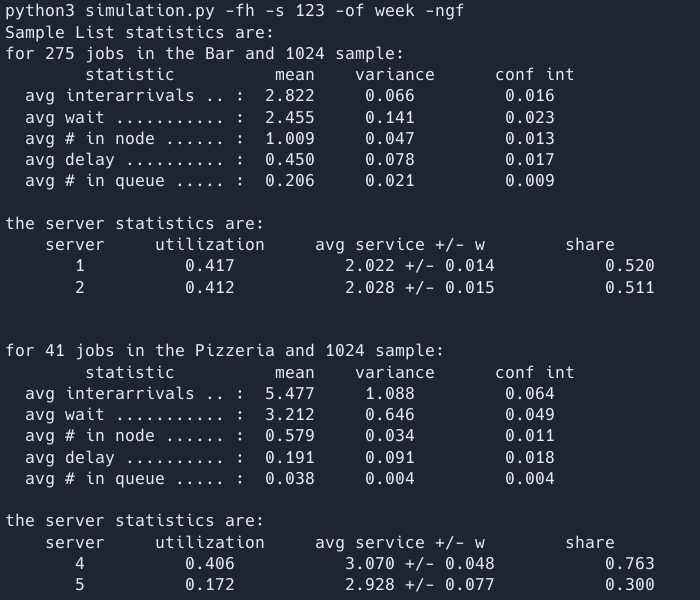
\includegraphics[width=0.8\textwidth]{finite_horizont_output_week_ngf}

\textit{Week day - senza fattore gaussiano}
\end{figure}
\end{minipage}
\begin{minipage}{0.5\textwidth}
\begin{figure}[H]
\centering
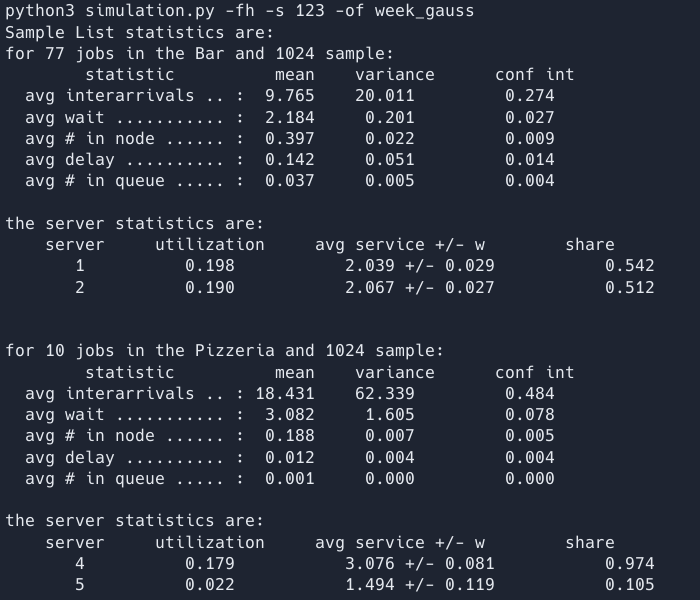
\includegraphics[width=0.8\textwidth]{finite_horizont_output_week_g}

\textit{Week day - con fattore gaussiano}
\end{figure}
\end{minipage}

\begin{minipage}{0.5\textwidth}
\begin{figure}[H]
\centering
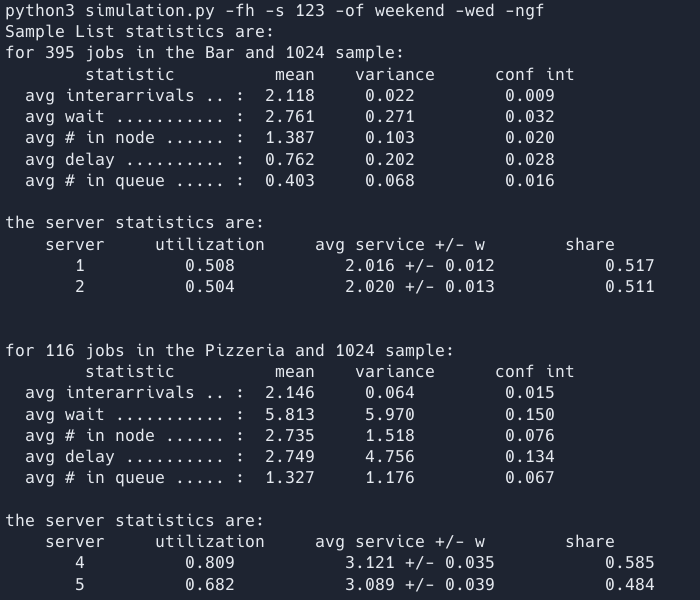
\includegraphics[width=0.8\textwidth]{finite_horizont_output_weekend_ngf}

\textit{Weekend day - senza fattore gaussiano}
\end{figure}
\end{minipage}
\begin{minipage}{0.5\textwidth}
\begin{figure}[H]
\centering
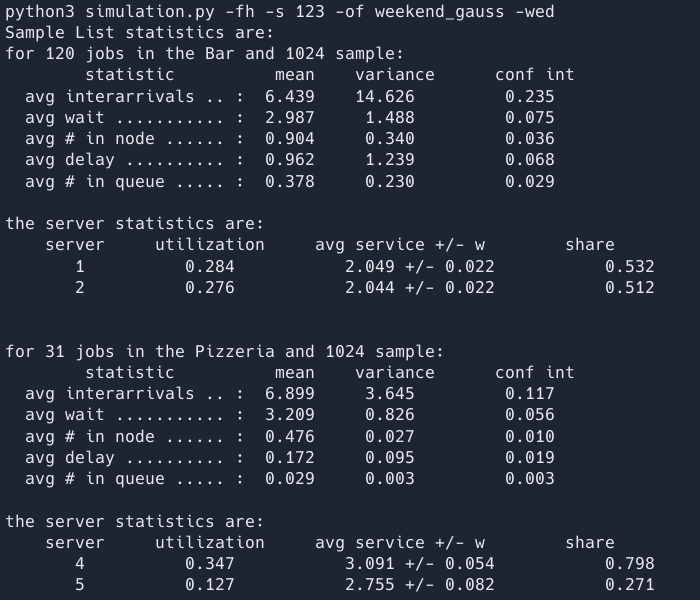
\includegraphics[width=0.8\textwidth]{finite_horizont_output_weekend_g}

\textit{Weekend day - con fattore gaussiano}
\end{figure}
\end{minipage}
\bigskip

Il numero di job riportati nelle immagini precedenti corrisponde alla media dei job processati nei vari \textit{run}, ed è il valore che verrà utilizzato successivamente come numero di richieste giornaliere nell'analisi dei costi. Il calcolo è stata effettuato su base mensile (4 settimane), e perciò le grandezze giornaliere sono state convertite; le configurazioni usate sono quelle di default presenti nel file \key{configurations/Config.py}.

\subsection{Analisi delle spese}
\begin{table}[H]
\centering
\begin{tabular}{|c|c|c|}
\hline
\cellcolor{cellcolor}Spesa & \cellcolor{cellcolor}Valore & \cellcolor{cellcolor}Contributo mensile \\
\hline
\hline
Baristi & 40 $\mbox{\euro}$ al giorno per barista & $40 \cdot 28 \cdot 2 = 2240\ \mbox{\euro}$ al mese \\
\hline
Pizzaiolo & 50 $\mbox{\euro}$ al giorno & $50 \cdot 28 = 1400\ \mbox{\euro}$  al mese\\
\hline
Bollette & 2750 $\mbox{\euro}$ al mese & 2750 $\mbox{\euro}$ al mese \\
\hline
Affitto & 1500 $\mbox{\euro}$ al mese & 1500 $\mbox{\euro}$ al mese\\
\hline
Fornitori & 2000 $\mbox{\euro}$ al mese & 2000 $\mbox{\euro}$ al mese\\
\hline
\hline
%\multicolumn{2}{|c|}{Totale} & \cellcolor{red!40} \textcolor[RGB]{230,10,10}{12970 $\mbox{\euro}$}\\
\multicolumn{2}{|c|}{Totale} & \cellcolor{red!40} 12970 $\mbox{\euro}$\\
\hline

\end{tabular}
\end{table}

\subsection{Analisi dei guadagni}
\begin{adjustbox}{width=\textwidth}
\begin{tabular}{|c|c|c|c|c|}
\hline
\cellcolor{cellcolor}Tipo richiesta & \cellcolor{cellcolor}Richieste \textit{week} & \cellcolor{cellcolor}Richieste \textit{weekend} & \cellcolor{cellcolor}Guadagno & \cellcolor{cellcolor}Contributo mensile \\
\hline
\noalign{\vspace{0.5ex}}
\hline
Tipo B & 275 & $5\ \mbox{\euro}$ a richiesta & \makecell{$275 \cdot 5\ \mbox{\euro} \cdot 5 \cdot 4 =$ \\ $27500\ \mbox{\euro}$ al mese }\\
\hline
Tipo P & 41 & $10\ \mbox{\euro}$ a richiesta & \makecell{$41 \cdot 10\ \mbox{\euro} \cdot 2 \cdot 4 =$ \\ $820\ \mbox{\euro}$} \\

\hline
\hline

%\multicolumn{2}{|c|}{Totale} & \cellcolor{red!40} \textcolor[RGB]{230,10,10}{12970 $\mbox{\euro}$}\\
\multicolumn{4}{|c|}{Totale} & \cellcolor{green!40} 12970 $\mbox{\euro}$\\
\hline

\end{tabular}
\end{adjustbox}


\section{Conclusioni}
Come si nota dai risultati ottenuti, a parte per qualche errore di
approssimazione, i risultati della simulazione tendono a quelli
teorici.\\
I risultati dell'analisi mostrano che il numero migliore di baristi da assumere
è 2: infatti questo è il numero minimo con cui si riesce a rispettare il
vincolo sul tempo di risposta, anche se il guadagno sarebbe stato maggiore con
$m = 1$. Continuando invece ad aumentare il numero di baristi, il guadagno
diminuisce sempre di più, mentre migliorano i tempi di risposta:
\bigskip 
\begin{center}
\begin{tabular}{ |c|c|c| }
  \hline
  $m$ & $E[T\textsubscript{S}]$ & $r(\tau)$ \\
  \hline
  \hline
  1 & 5.53 min & 3070.10 $\mbox{\euro}\text{ al mese}$ \\
  \hline
  2 & 2.18 min & 1853.43 $\mbox{\euro}\text{ al mese}$ \\
  \hline
  3 & 2.02 min & 636.76 $\mbox{\euro}\text{ al mese}$ \\
  \hline
  4 & 2.00 min & -579.90 $\mbox{\euro}\text{ al mese}$ \\
  \hline
\end{tabular}
\end{center}

Si può notare che, al crescere di $m$, la differenza dei tempi con il caso $m
- 1$ è sempre minore: questo si può spiegare considerando che i tassi di arrivo
non sono stati cambiati: aumentando $m$, quindi, si va a diminuire il tempo di
coda di ogni job, che tende quindi a 0.

%
%\section{Immagini}
%
%\target{rappresentazione grafica gaussiane}
%\subsection{Distribuzioni gaussiane per gli arrivi}
%\[
%y=\frac{1}{\sqrt{2\pi}\sigma}e^\frac{-(x-\mu)^2}{2\sigma^2}
%\]
%
%\begin{figure}[H]
%\centering 
%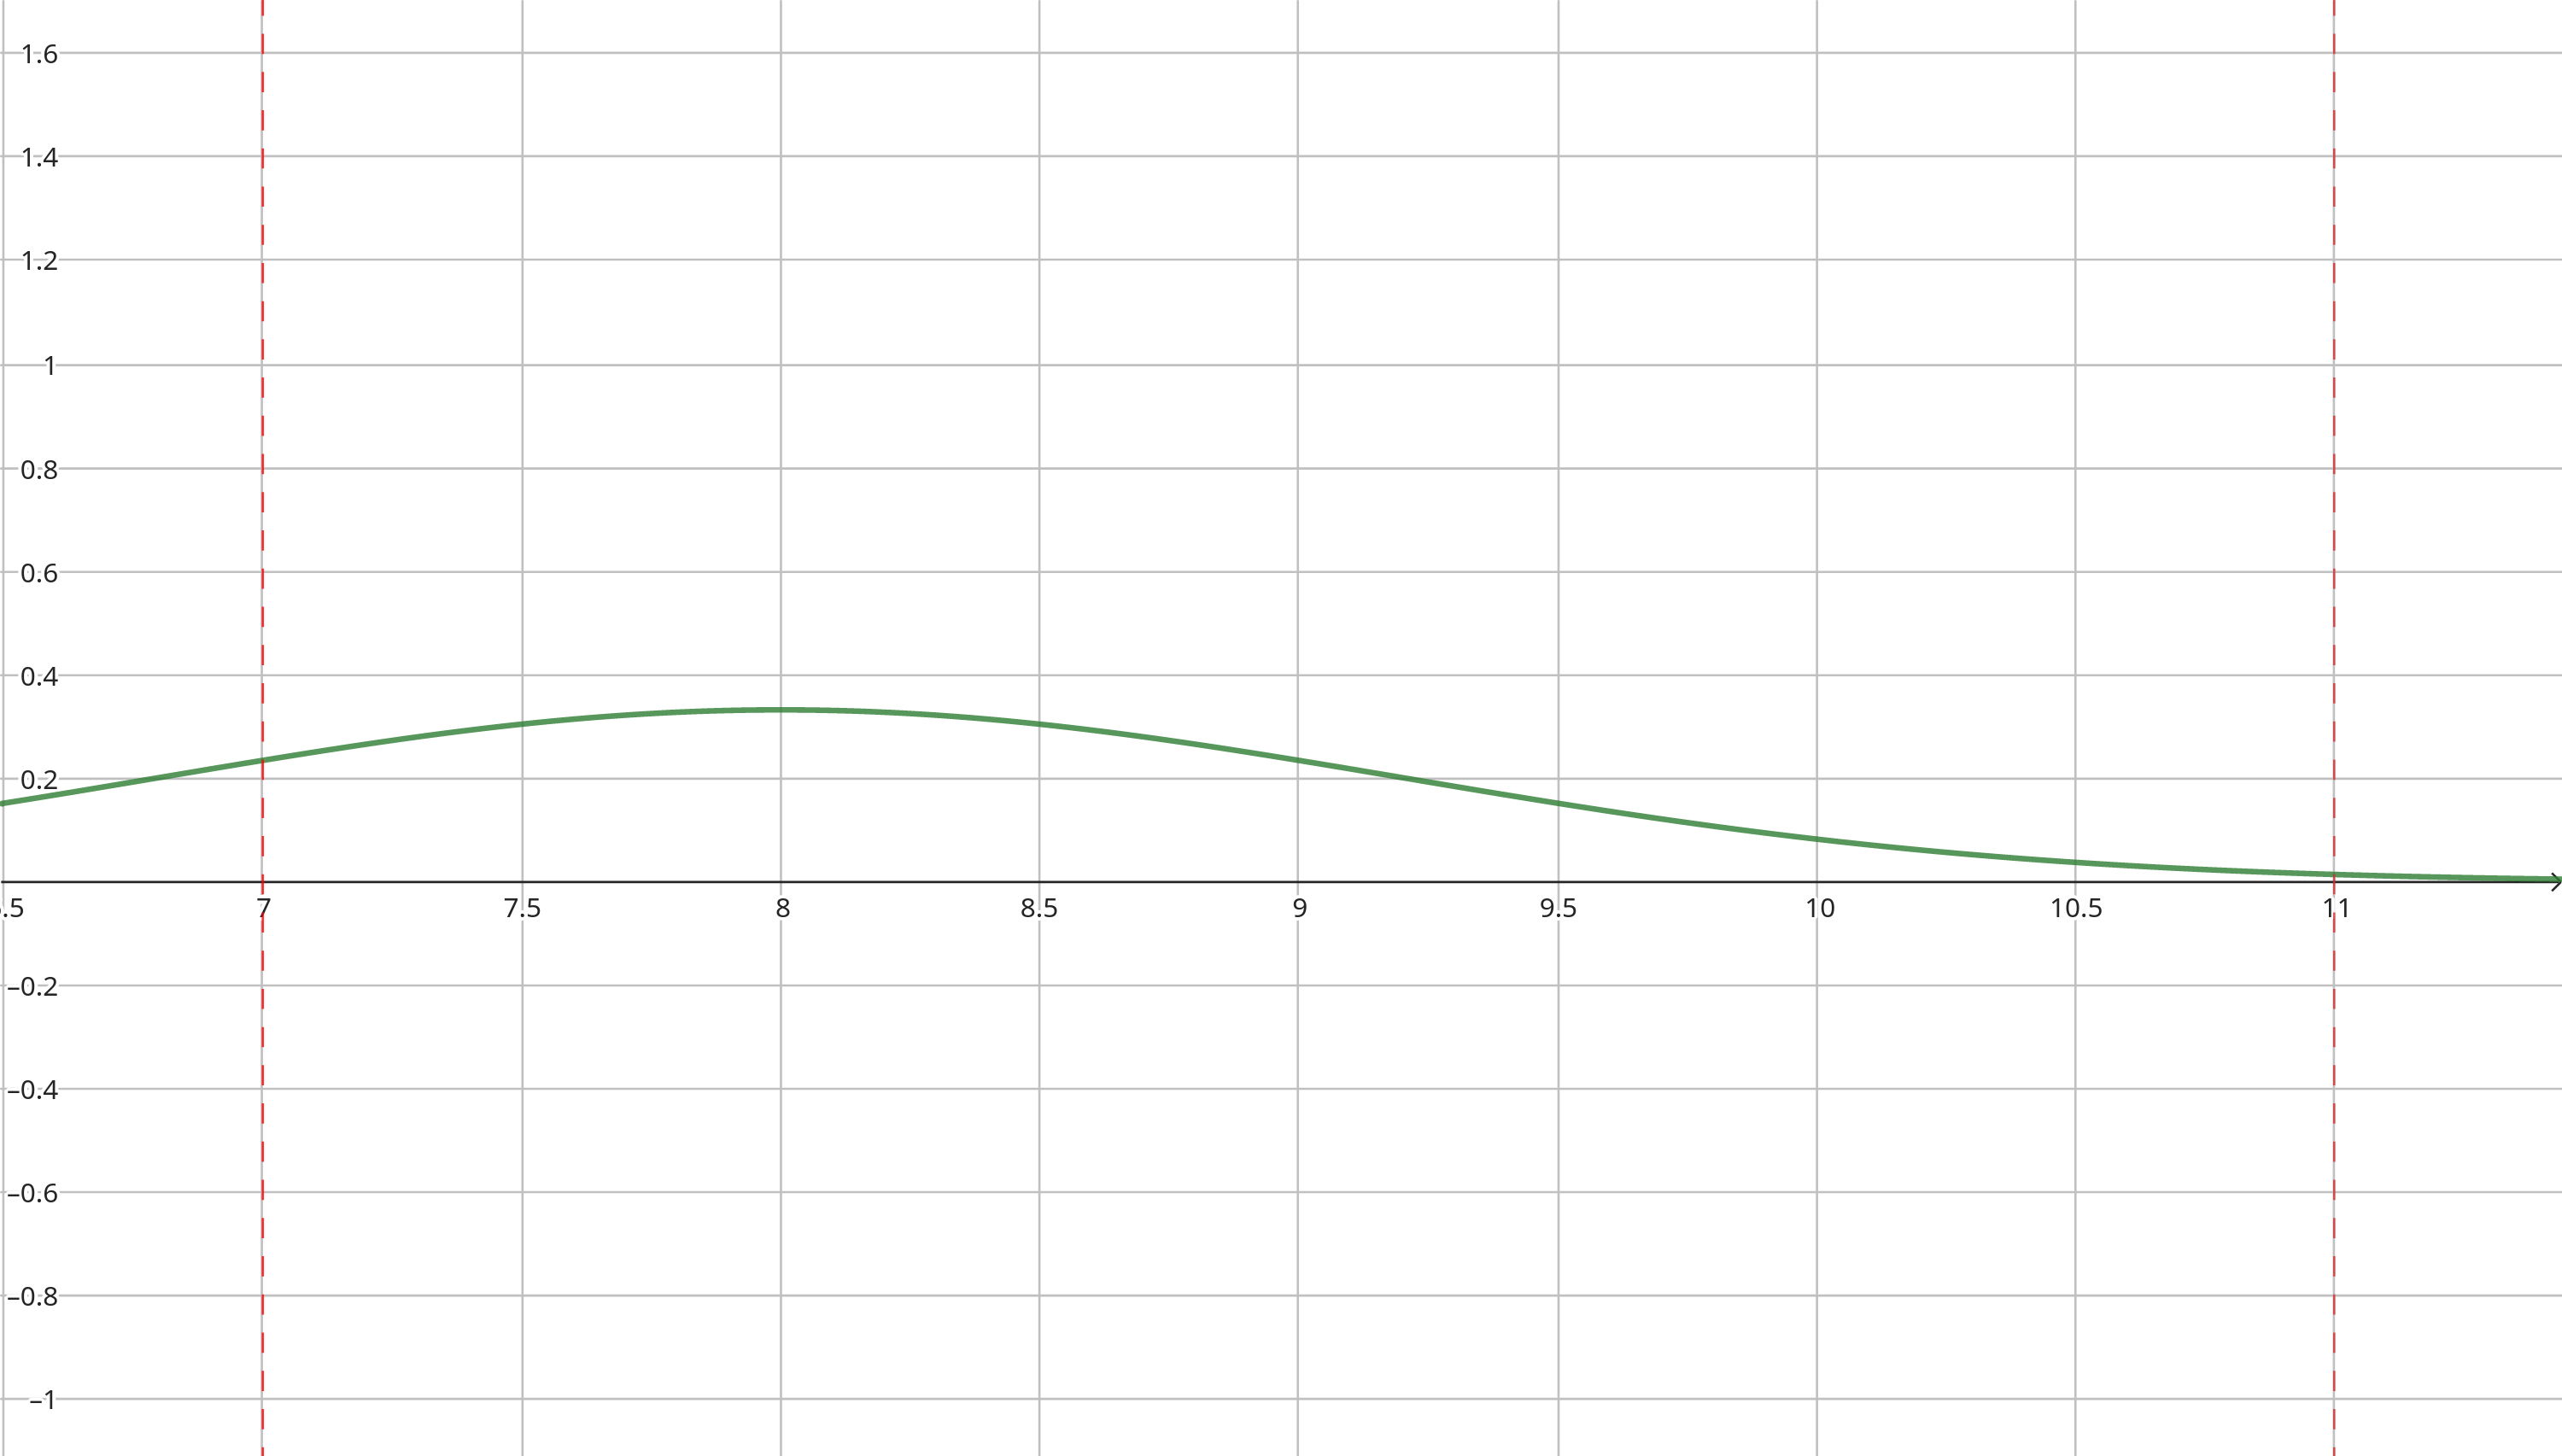
\includegraphics[width=0.8\textwidth]{7-11-gaussian}
%\bigskip
%
%\textit{Fascia oraria: 07:00 $\rightarrow$ 11:00}
%\[ \mu = 8;\ \sigma = 1.2 \]
%\end{figure}
%
%
%\begin{figure}[H]
%\centering 
%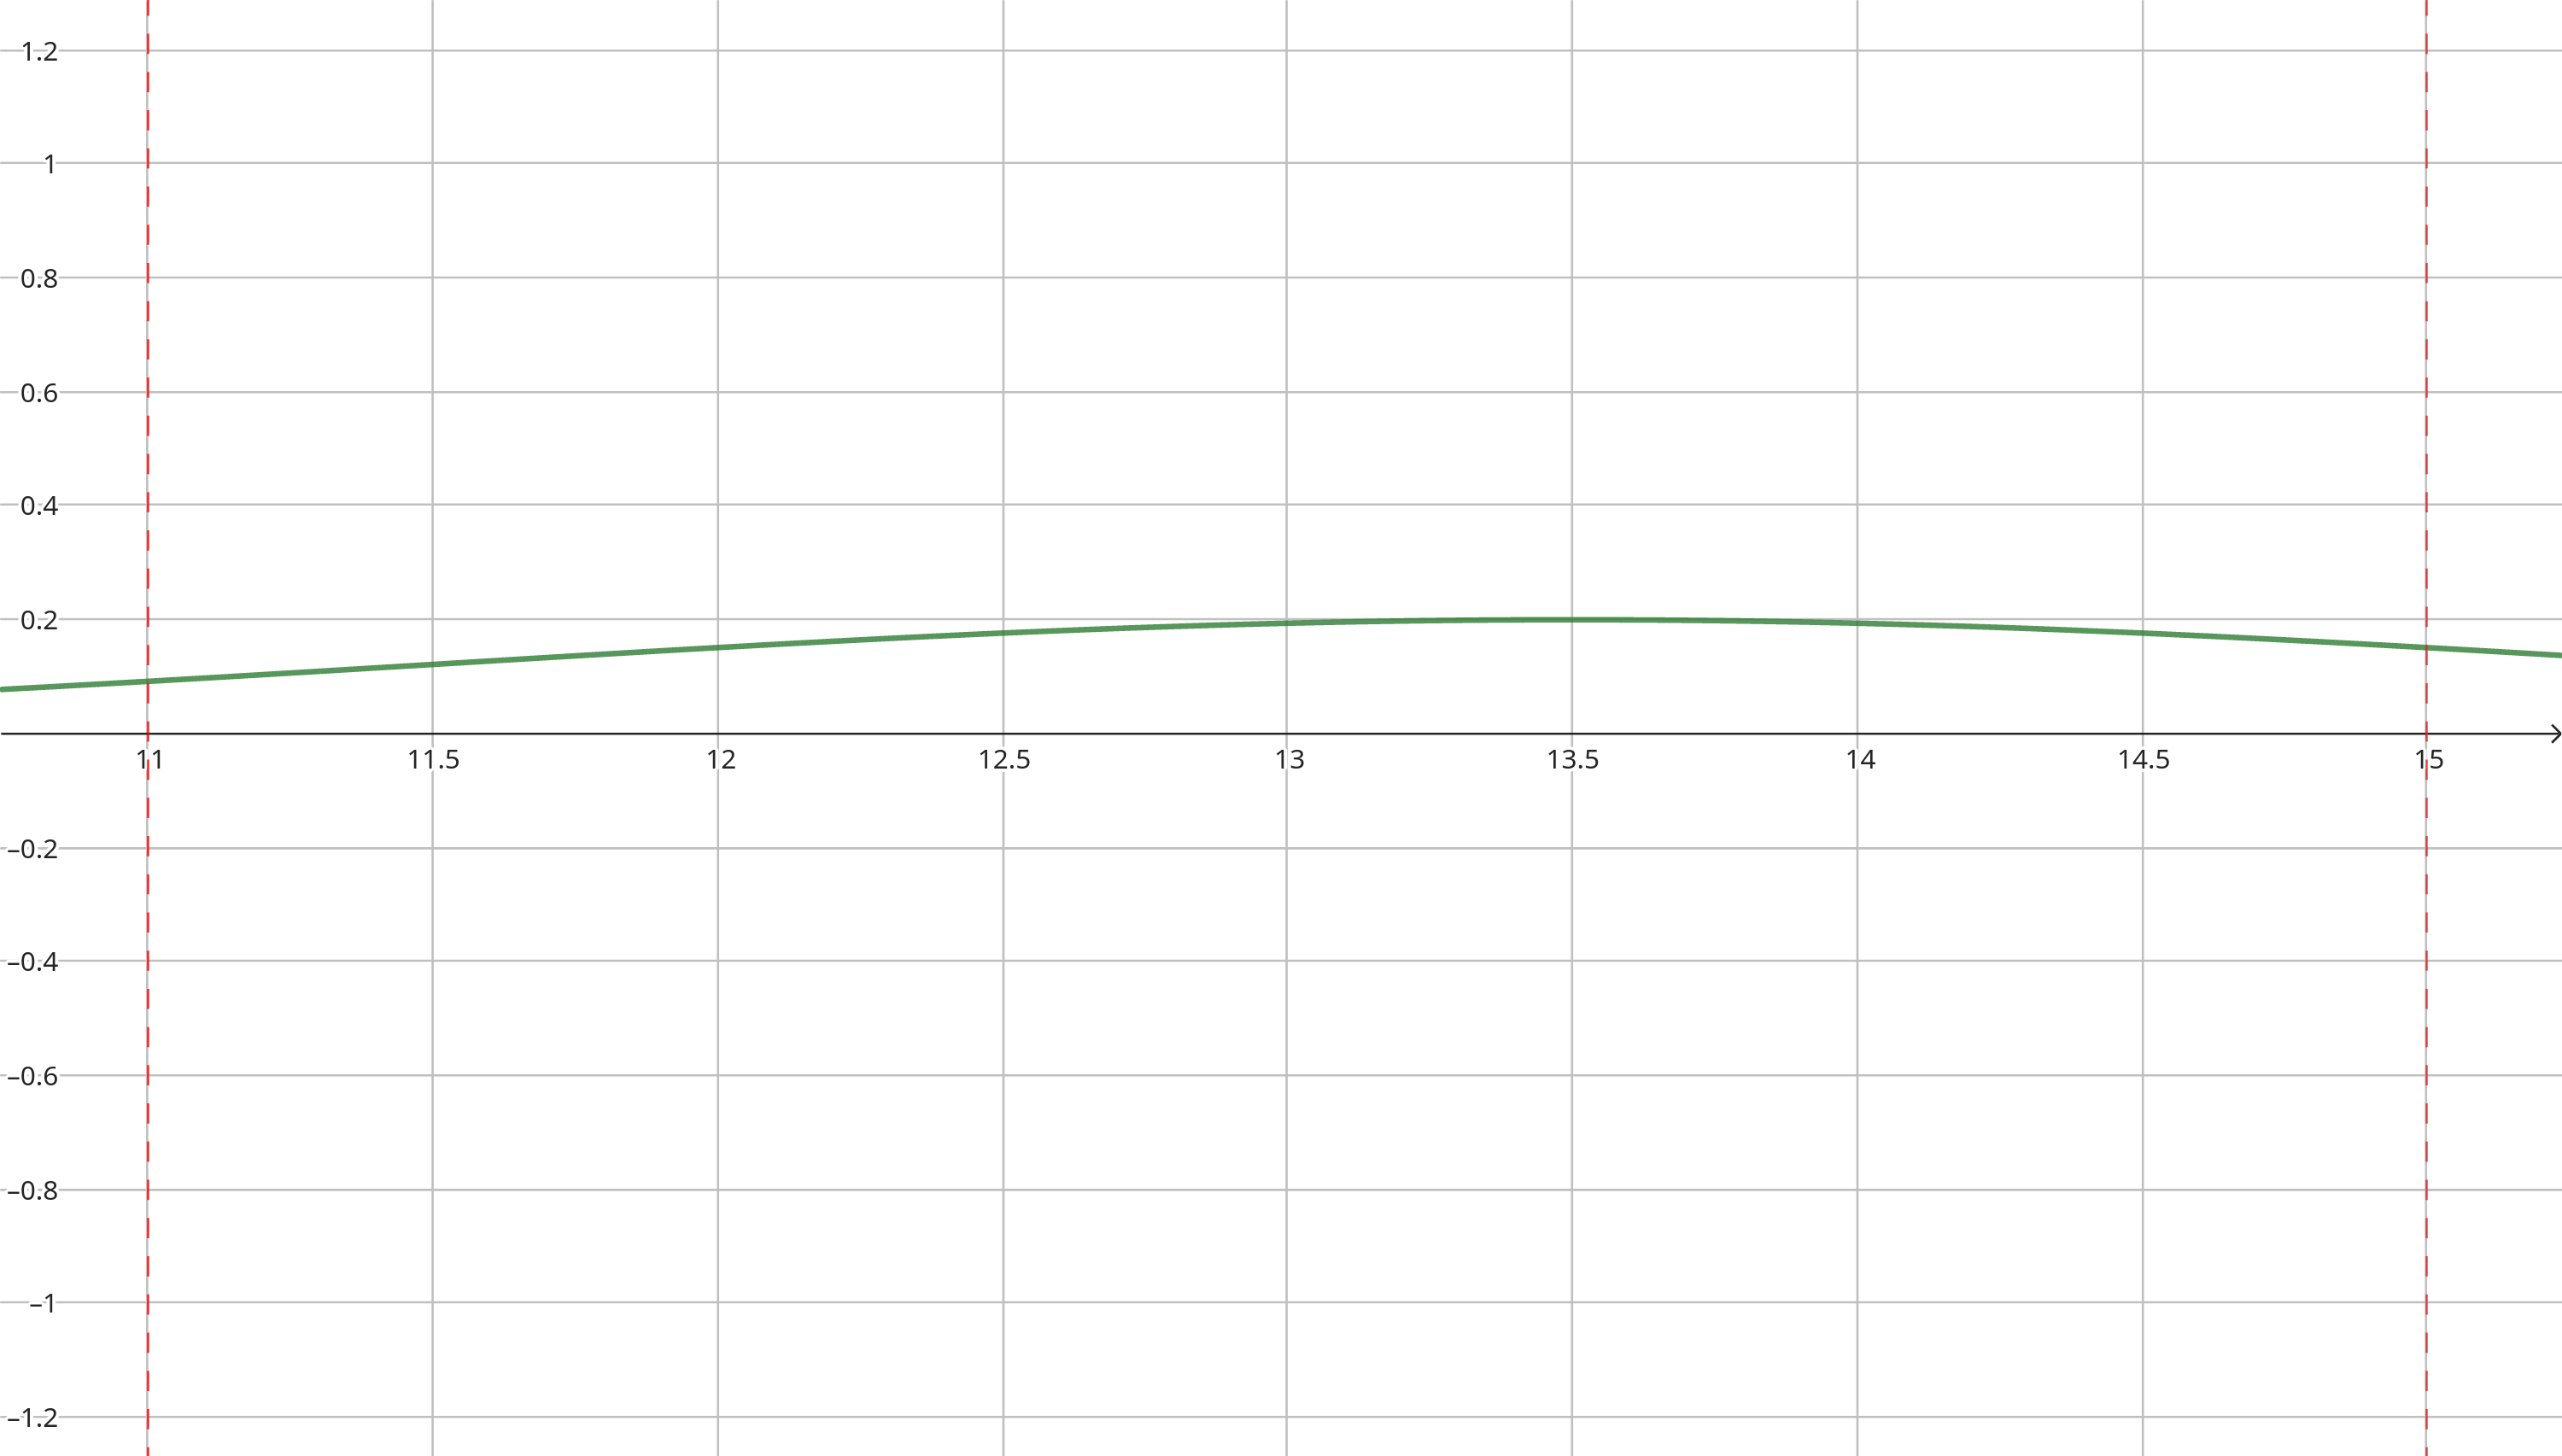
\includegraphics[width=0.8\textwidth]{11-15-gaussian}\bigskip
%
%\textit{Fascia oraria: 11:00 $\rightarrow$ 15:00}
%\[ \mu = 13.5;\ \sigma = 2 \]
%\end{figure}
%
%
%\begin{figure}[H]
%\centering 
%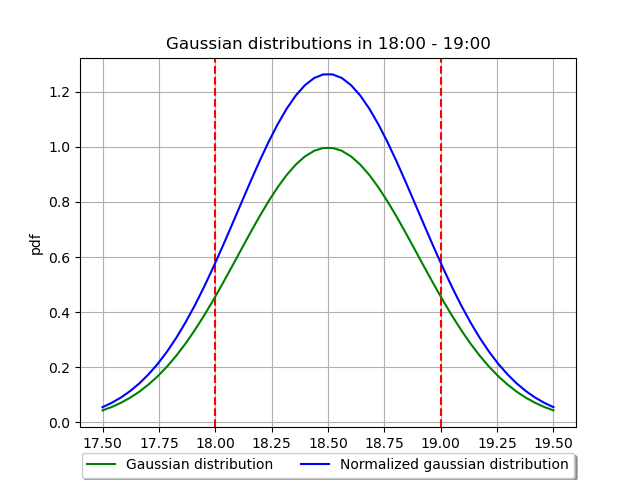
\includegraphics[width=0.8\textwidth]{18-19-gaussian}\bigskip
%
%\textit{Fascia oraria: 18:00 $\rightarrow$ 19:00}
%\[ \mu = 18.5;\ \sigma = 0.4 \]
%\end{figure}
%
%\begin{figure}[H]
%\centering 
%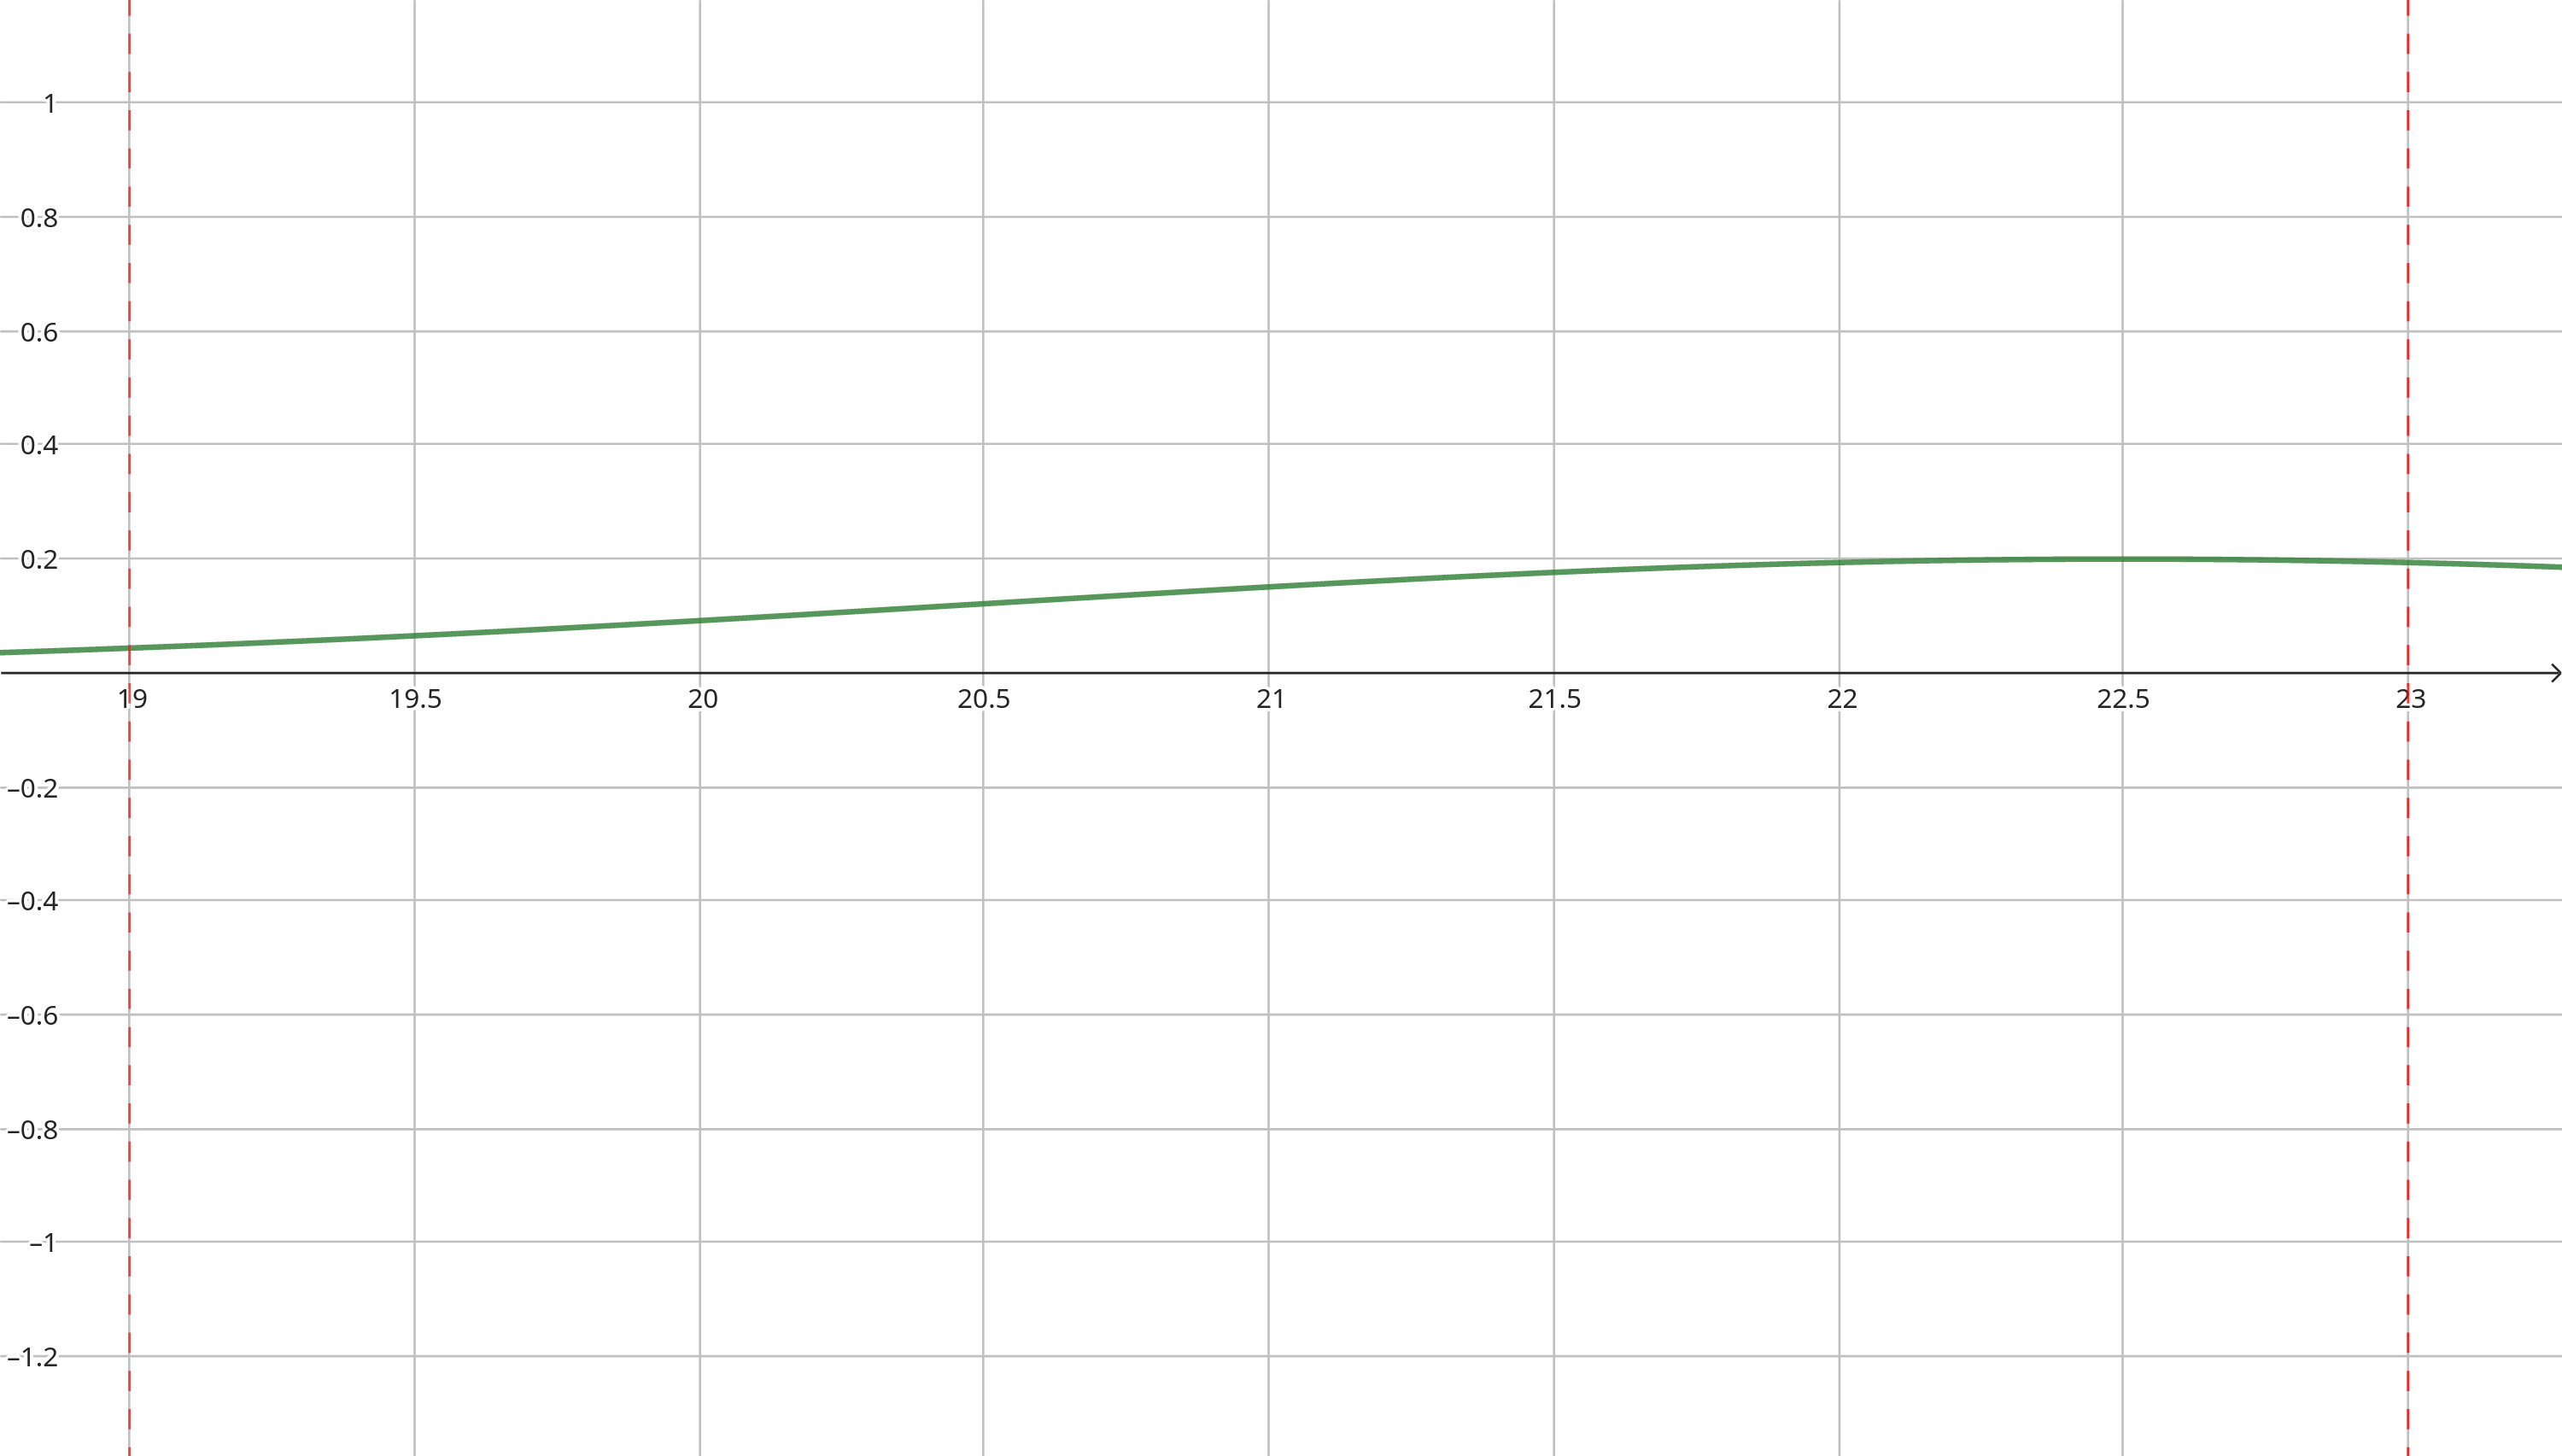
\includegraphics[width=0.8\textwidth]{19-23-gaussian}\bigskip
%
%\textit{Fascia oraria: 19:00 $\rightarrow$ 23:00, bar}
%\[ \mu = 22.5;\ \sigma = 2 \]
%\end{figure}
%
%\begin{figure}[H]
%\centering 
%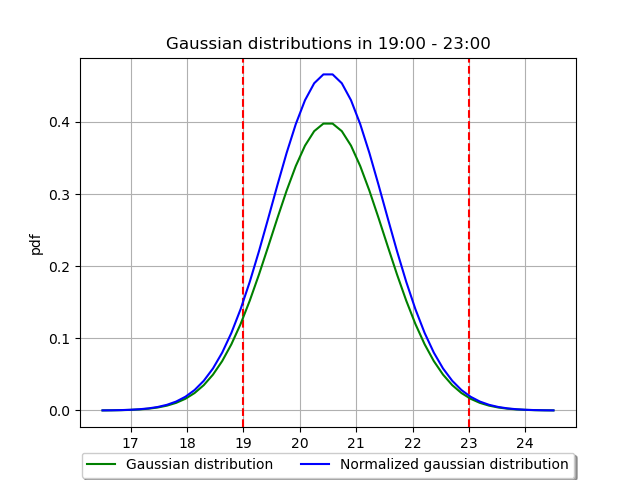
\includegraphics[width=0.8\textwidth]{19-23-gaussian-pizza}\bigskip
%
%\textit{Fascia oraria: 19:00 $\rightarrow$ 23:00, pizzeria}
%\[ \mu = 20.5;\ \sigma = 1 \]
%\end{figure}
%
%\begin{figure}[H]
%\centering 
%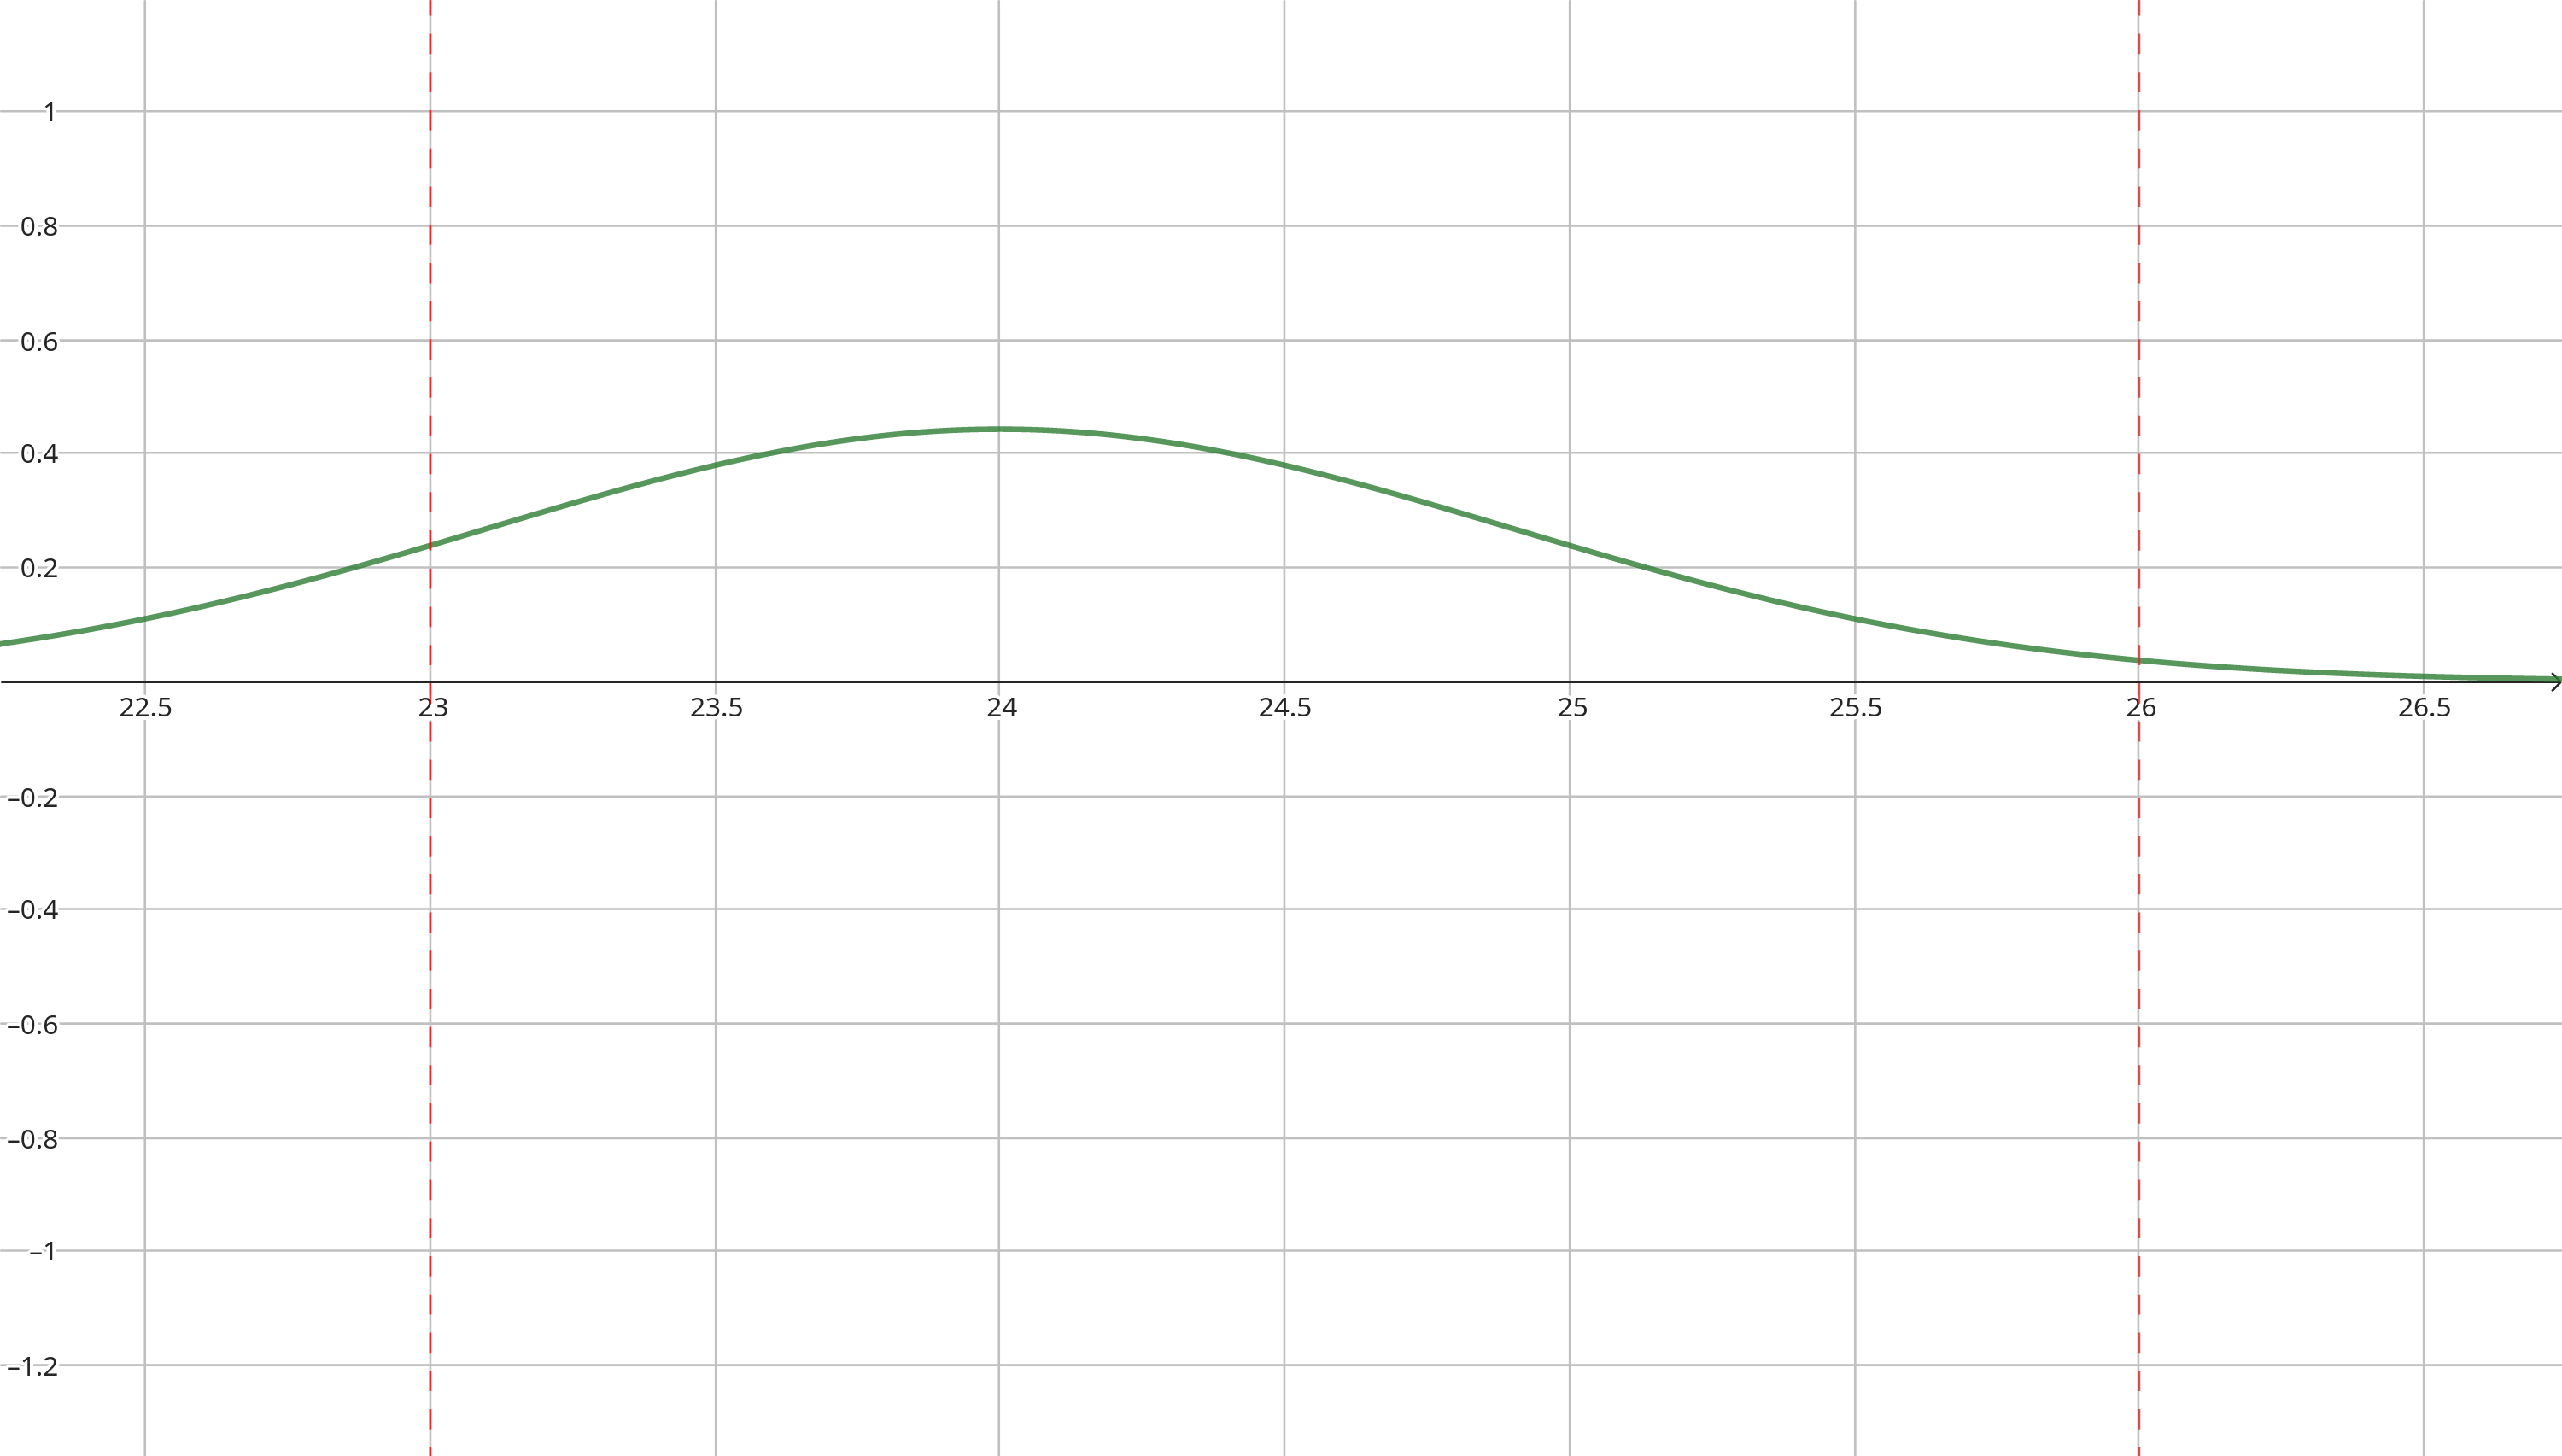
\includegraphics[width=0.8\textwidth]{23-02-gaussian}\bigskip
%
%\textit{Fascia oraria: 23:00 $\rightarrow$ 02:00}
%\[ \mu = 24;\ \sigma = 0.9 \]
%\end{figure}
%
%%__________________________________________
%
%
%\subsection{Interarrivi}
%\subsubsection{Week - orizzonte infinito}
%\target{interarrivo infinito week slot 0}
%\paragraph{Slot 0}
%\subparagraph*{}
%\begin{figure}[H]
%\centering 
%\includegraphics[width=0.8\textwidth]{/infinite/slot_0/avgInterarrivals/week_B_0}
%\centering \textit{}
%\end{figure}
%
%\target{interarrivo infinito week slot 1}
%\paragraph{Slot 1}
%\subparagraph*{}
%\begin{figure}[H]
%\centering 
%\includegraphics[width=0.8\textwidth]{/infinite/slot_1/avgInterarrivals/week_B_1}
%\centering \textit{}
%\end{figure}
%
%\target{interarrivo infinito week slot 3}
%\paragraph{Slot 3}
%\subparagraph*{}
%\begin{figure}[H]
%\centering 
%\includegraphics[width=0.8\textwidth]{/infinite/slot_3/avgInterarrivals/week_B_3}
%\centering \textit{}
%\end{figure}
%
%\target{interarrivo infinito week slot 4}
%\paragraph{Slot 4}
%\subparagraph*{}
%\begin{figure}[H]
%\centering 
%\includegraphics[width=0.8\textwidth]{/infinite/slot_4/avgInterarrivals/week_B_4}
%\centering \textit{}
%\end{figure}
%
%\target{interarrivo infinito week slot 5}
%\paragraph{Slot 5}
%\subparagraph*{}
%\begin{figure}[H]
%\centering 
%\includegraphics[width=0.8\textwidth]{/infinite/slot_5/avgInterarrivals/week_B_5}
%\centering \textit{}
%\end{figure}
%
%\paragraph{P}
%\target{interarrivo infinito week P}
%\subparagraph*{}
%\begin{figure}[H]
%\centering 
%\includegraphics[width=0.8\textwidth]{/infinite/slot_4/avgInterarrivals/week_P_4}
%\centering \textit{}
%\end{figure}
%
%
%\subsubsection{Weekend - orizzonte infinito}
%\target{interarrivo infinito weekend slot 0}
%\paragraph{Slot 0}
%\subparagraph*{}
%\begin{figure}[H]
%\centering 
%\includegraphics[width=0.8\textwidth]{/infinite/slot_0/avgInterarrivals/weekend_B_0}
%\centering \textit{}
%\end{figure}
%
%\paragraph{Slot 1}
%\target{interarrivo infinito weekend slot 1}
%\subparagraph*{}
%\begin{figure}[H]
%\centering 
%\includegraphics[width=0.8\textwidth]{/infinite/slot_1/avgInterarrivals/weekend_B_1}
%\centering \textit{}
%\end{figure}
%
%\paragraph{Slot 3}
%\target{interarrivo infinito weekend slot 3}
%\subparagraph*{}
%\begin{figure}[H]
%\centering 
%\includegraphics[width=0.8\textwidth]{/infinite/slot_3/avgInterarrivals/weekend_B_3}
%\centering \textit{}
%\end{figure}
%
%\paragraph{Slot 4}
%\target{interarrivo infinito weekend slot 4}
%\subparagraph*{}
%\begin{figure}[H]
%\centering 
%\includegraphics[width=0.8\textwidth]{/infinite/slot_4/avgInterarrivals/weekend_B_4}
%\centering \textit{}
%\end{figure}
%
%\paragraph{Slot 5}
%\target{interarrivo infinito weekend slot 5}
%\subparagraph*{}
%\begin{figure}[H]
%\centering 
%\includegraphics[width=0.8\textwidth]{/infinite/slot_5/avgInterarrivals/weekend_B_5}
%\centering \textit{}
%\end{figure}
%
%\paragraph{P}
%\target{interarrivo infinito weekend P}
%\subparagraph*{}
%\begin{figure}[H]
%\centering 
%\includegraphics[width=0.8\textwidth]{/infinite/slot_4/avgInterarrivals/weekend_P_4}
%\centering \textit{}
%\end{figure}
%%__________________________________________
%
%
%
%\subsection{Attesa}
%\subsubsection{Week - orizzonte infinito}
%\target{attesa infinita week slot 0}
%\paragraph{Slot 0}
%\subparagraph*{}
%\begin{figure}[H]
%\centering 
%\includegraphics[width=0.8\textwidth]{/infinite/slot_0/avgWaits/week_B_0}
%\centering \textit{}
%\end{figure}
%
%\target{attesa infinita week slot 1}
%\paragraph{Slot 1}
%\subparagraph*{}
%\begin{figure}[H]
%\centering 
%\includegraphics[width=0.8\textwidth]{/infinite/slot_1/avgWaits/week_B_1}
%\centering \textit{}
%\end{figure}
%
%\target{attesa infinita week slot 3}
%\paragraph{Slot 3}
%\subparagraph*{}
%\begin{figure}[H]
%\centering 
%\includegraphics[width=0.8\textwidth]{/infinite/slot_3/avgWaits/week_B_3}
%\centering \textit{}
%\end{figure}
%
%\target{attesa infinita week slot 4}
%\paragraph{Slot 4}
%\subparagraph*{}
%\begin{figure}[H]
%\centering 
%\includegraphics[width=0.8\textwidth]{/infinite/slot_4/avgWaits/week_B_4}
%\centering \textit{}
%\end{figure}
%
%\target{attesa infinita week slot 5}
%\paragraph{Slot 5}
%\subparagraph*{}
%\begin{figure}[H]
%\centering 
%\includegraphics[width=0.8\textwidth]{/infinite/slot_5/avgWaits/week_B_5}
%\centering \textit{}
%\end{figure}
%
%\paragraph{P}
%\target{attesa infinita week P}
%\subparagraph*{}
%\begin{figure}[H]
%\centering 
%\includegraphics[width=0.8\textwidth]{/infinite/slot_4/avgWaits/week_P_4}
%\centering \textit{}
%\end{figure}
%
%
%\subsubsection{Weekend - orizzonte infinito}
%\target{attesa infinita weekend slot 0}
%\paragraph{Slot 0}
%\subparagraph*{}
%\begin{figure}[H]
%\centering 
%\includegraphics[width=0.8\textwidth]{/infinite/slot_0/avgWaits/weekend_B_0}
%\centering \textit{}
%\end{figure}
%
%\target{attesa infinita weekend slot 1}
%\paragraph{Slot 1}
%\subparagraph*{}
%\begin{figure}[H]
%\centering 
%\includegraphics[width=0.8\textwidth]{/infinite/slot_1/avgWaits/weekend_B_1}
%\centering \textit{}
%\end{figure}
%
%\target{attesa infinita weekend slot 3}
%\paragraph{Slot 3}
%\subparagraph*{}
%\begin{figure}[H]
%\centering 
%\includegraphics[width=0.8\textwidth]{/infinite/slot_3/avgWaits/weekend_B_3}
%\centering \textit{}
%\end{figure}
%
%\target{attesa infinita weekend slot 4}
%\paragraph{Slot 4}
%\subparagraph*{}
%\begin{figure}[H]
%\centering 
%\includegraphics[width=0.8\textwidth]{/infinite/slot_4/avgWaits/weekend_B_4}
%\centering \textit{}
%\end{figure}
%
%\target{attesa infinita weekend slot 5}
%\paragraph{Slot 5}
%\subparagraph*{}
%\begin{figure}[H]
%\centering 
%\includegraphics[width=0.8\textwidth]{/infinite/slot_5/avgWaits/weekend_B_5}
%\centering \textit{}
%\end{figure}
%
%\paragraph{P}
%\target{attesa infinita weekend P}
%\subparagraph*{}
%\begin{figure}[H]
%\centering 
%\includegraphics[width=0.8\textwidth]{/infinite/slot_4/avgWaits/weekend_P_4}
%\centering \textit{}
%\end{figure}
%
%
%\subsubsection{Week - orizzonte finito}
%\target{attesa finita week B no gau}
%\paragraph{Tipo B - no gaussian factor}
%\subparagraph*{}
%\begin{figure}[H]
%\centering 
%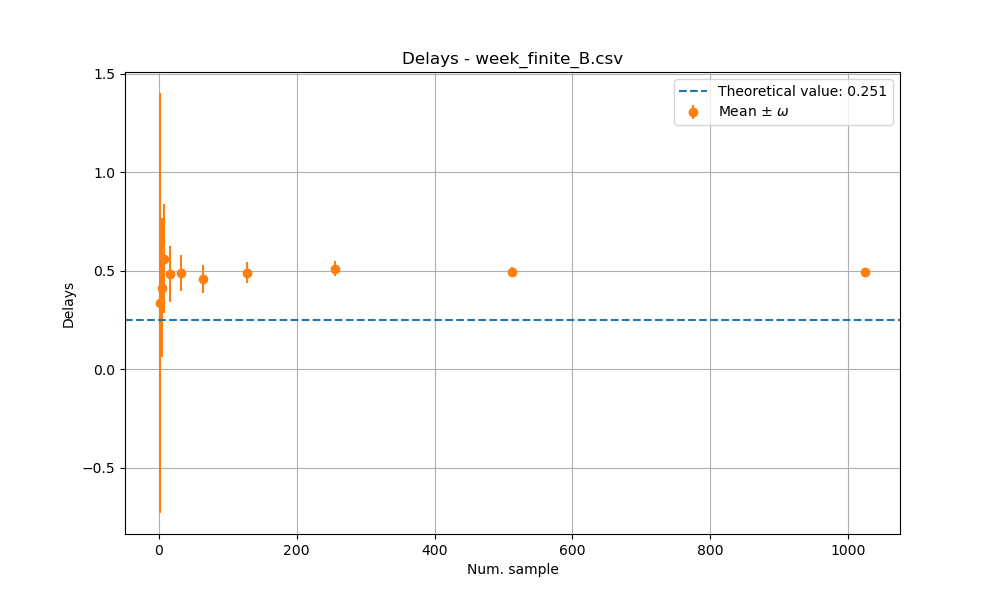
\includegraphics[width=0.8\textwidth]{/finite/avgWaits/week_B}
%\centering \textit{}
%\end{figure}
%
%\target{attesa finita week P no gau}
%\paragraph{Tipo P - no gaussian factor}
%\subparagraph*{}
%\begin{figure}[H]
%\centering 
%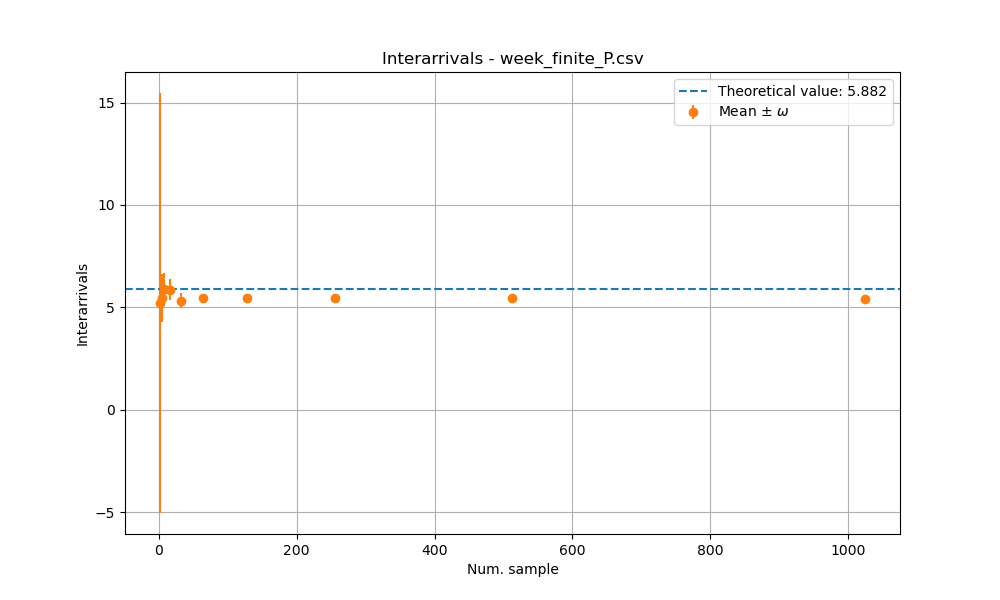
\includegraphics[width=0.8\textwidth]{/finite/avgWaits/week_P}
%\centering \textit{}
%\end{figure}
%
%\target{attesa finita week B gau}
%\paragraph{Tipo B - gaussian factor}
%\subparagraph*{}
%\begin{figure}[H]
%\centering 
%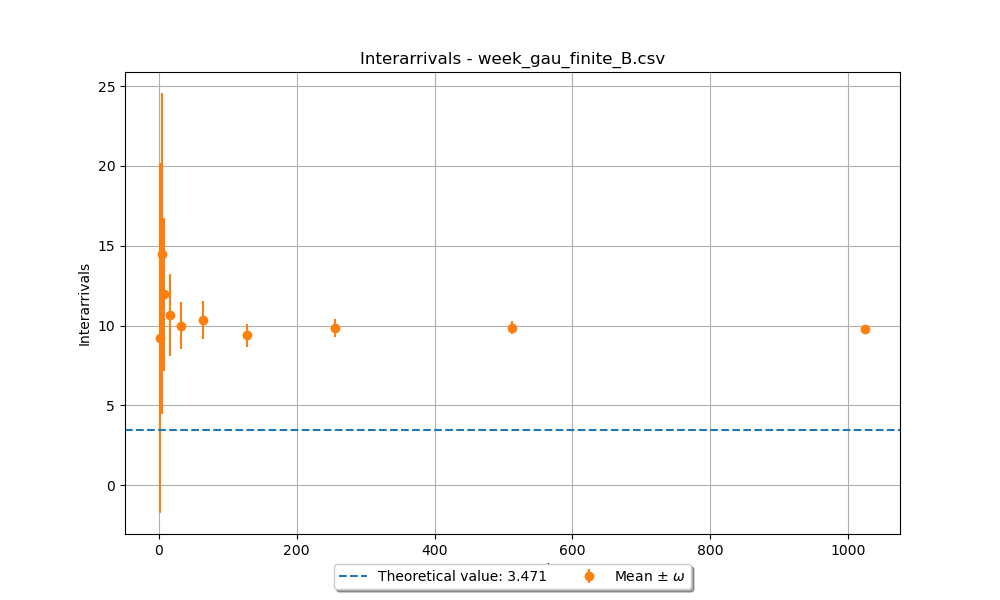
\includegraphics[width=0.8\textwidth]{/finite/avgWaits/week_B_gau}
%\centering \textit{}
%\end{figure}
%
%\target{attesa finita week P gau}
%\paragraph{Tipo P - gaussian factor}
%\subparagraph*{}
%\begin{figure}[H]
%\centering 
%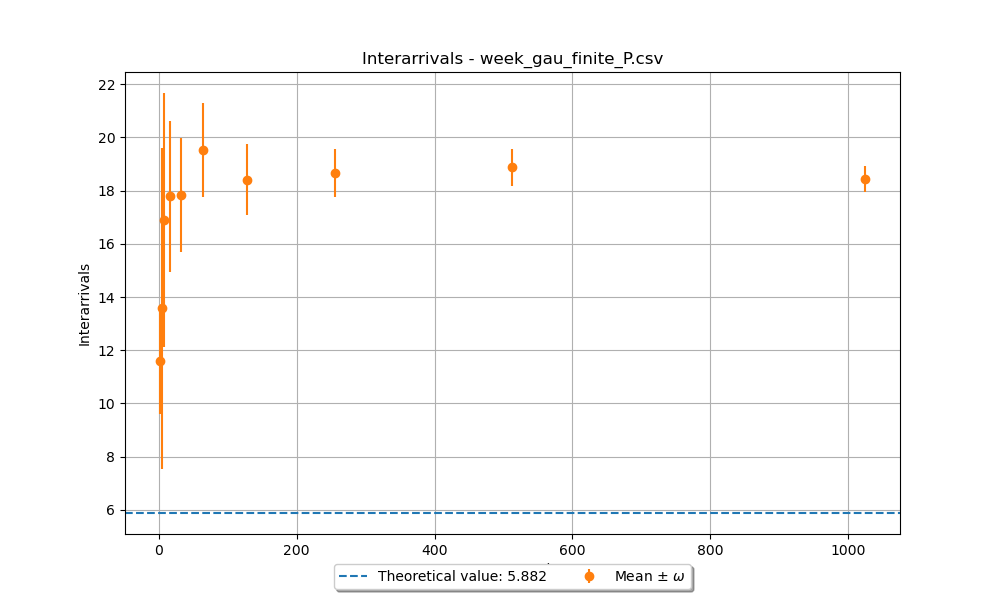
\includegraphics[width=0.8\textwidth]{/finite/avgWaits/week_P_gau}
%\centering \textit{}
%\end{figure}
%
%
%
%\subsubsection{Weekend - orizzonte finito}
%\target{attesa finita weekend B no gau}
%\paragraph{Tipo B}
%\subparagraph*{}
%\begin{figure}[H]
%\centering 
%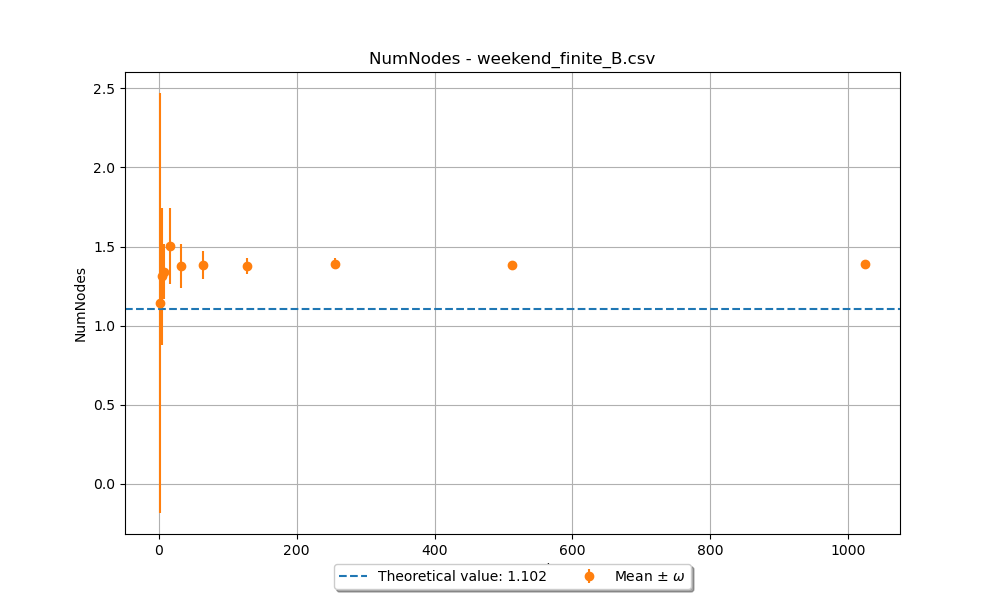
\includegraphics[width=0.8\textwidth]{/finite/avgWaits/weekend_B}
%\centering \textit{}
%\end{figure}
%
%\target{attesa finita weekend P no gau}
%\paragraph{Tipo P}
%\subparagraph*{}
%\begin{figure}[H]
%\centering 
%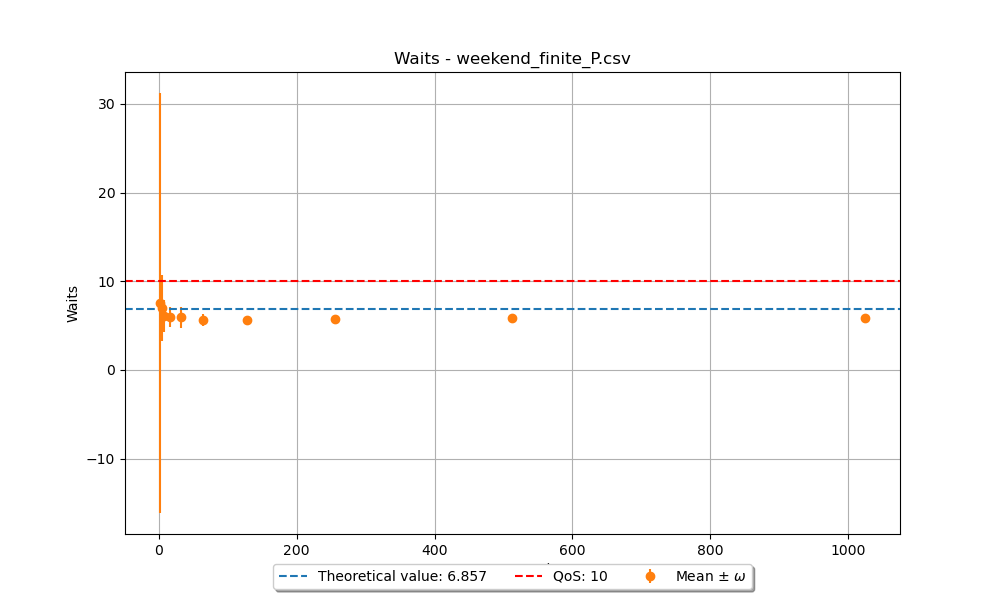
\includegraphics[width=0.8\textwidth]{/finite/avgWaits/weekend_P}
%\centering \textit{}
%\end{figure}
%
%\target{attesa finita weekend B gau}
%\paragraph{Tipo B - gaussian factor}
%\subparagraph*{}
%\begin{figure}[H]
%\centering 
%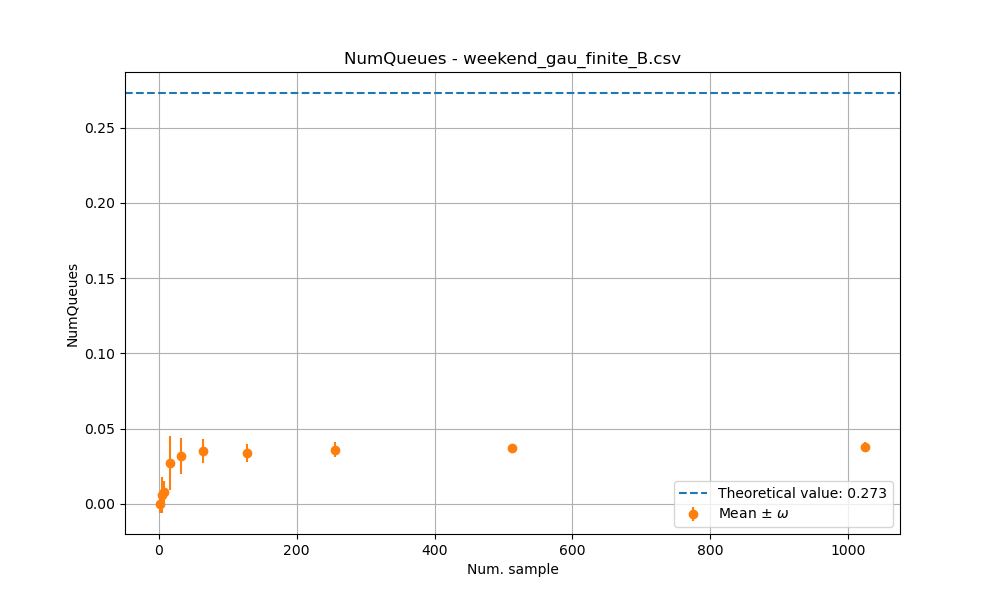
\includegraphics[width=0.8\textwidth]{/finite/avgWaits/weekend_B_gau}
%\centering \textit{}
%\end{figure}
%
%\target{attesa finita weekend P gau}
%\paragraph{Tipo P - gaussian factor}
%\subparagraph*{}
%\begin{figure}[H]
%\centering 
%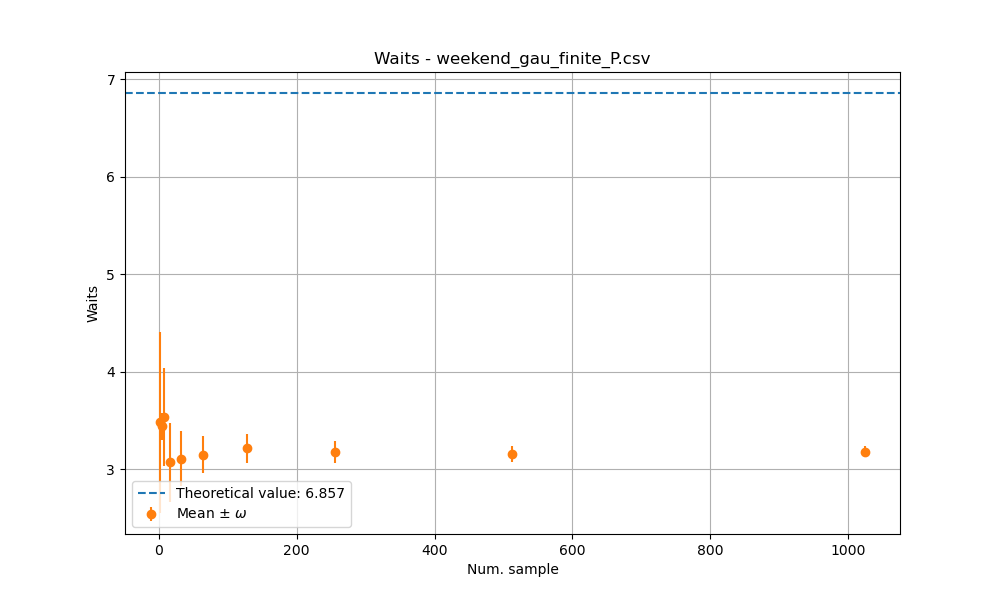
\includegraphics[width=0.8\textwidth]{/finite/avgWaits/weekend_P_gau}
%\centering \textit{}
%\end{figure}
%
%
%%__________________________________________
%
%\subsection{Popolazione nel centro}
%\subsubsection{Week - orizzonte infinito}
%\target{centro infinito week slot 0}
%\paragraph{Slot 0}
%\subparagraph*{}
%\begin{figure}[H]
%\centering 
%\includegraphics[width=0.8\textwidth]{/infinite/slot_0/avgNumNodes/week_B_0}
%\centering \textit{}
%\end{figure}
%
%\target{centro infinito week slot 1}
%\paragraph{Slot 1}
%\subparagraph*{}
%\begin{figure}[H]
%\centering 
%\includegraphics[width=0.8\textwidth]{/infinite/slot_1/avgNumNodes/week_B_1}
%\centering \textit{}
%\end{figure}
%
%\target{centro infinito week slot 3}
%\paragraph{Slot 3}
%\subparagraph*{}
%\begin{figure}[H]
%\centering 
%\includegraphics[width=0.8\textwidth]{/infinite/slot_3/avgNumNodes/week_B_3}
%\centering \textit{}
%\end{figure}
%
%\target{centro infinito week slot 4}
%\paragraph{Slot 4}
%\subparagraph*{}
%\begin{figure}[H]
%\centering 
%\includegraphics[width=0.8\textwidth]{/infinite/slot_4/avgNumNodes/week_B_4}
%\centering \textit{}
%\end{figure}
%
%\target{centro infinito week slot 5}
%\paragraph{Slot 5}
%\subparagraph*{}
%\begin{figure}[H]
%\centering 
%\includegraphics[width=0.8\textwidth]{/infinite/slot_5/avgNumNodes/week_B_5}
%\centering \textit{}
%\end{figure}
%
%\paragraph{P}
%\target{centro infinito week P}
%\subparagraph*{}
%\begin{figure}[H]
%\centering 
%\includegraphics[width=0.8\textwidth]{/infinite/slot_4/avgNumNodes/week_P_4}
%\centering \textit{}
%\end{figure}
%
%
%\subsubsection{Weekend - orizzonte infinito}
%\target{centro infinito weekend slot 0}
%\paragraph{Slot 0}
%\subparagraph*{}
%\begin{figure}[H]
%\centering 
%\includegraphics[width=0.8\textwidth]{/infinite/slot_0/avgNumNodes/weekend_B_0}
%\centering \textit{}
%\end{figure}
%
%\target{centro infinito weekend slot 1}
%\paragraph{Slot 1}
%\subparagraph*{}
%\begin{figure}[H]
%\centering 
%\includegraphics[width=0.8\textwidth]{/infinite/slot_1/avgNumNodes/weekend_B_1}
%\centering \textit{}
%\end{figure}
%
%\target{centro infinito weekend slot 3}
%\paragraph{Slot 3}
%\subparagraph*{}
%\begin{figure}[H]
%\centering 
%\includegraphics[width=0.8\textwidth]{/infinite/slot_3/avgNumNodes/weekend_B_3}
%\centering \textit{}
%\end{figure}
%
%\target{centro infinito weekend slot 4}
%\paragraph{Slot 4}
%\subparagraph*{}
%\begin{figure}[H]
%\centering 
%\includegraphics[width=0.8\textwidth]{/infinite/slot_4/avgNumNodes/weekend_B_4}
%\centering \textit{}
%\end{figure}
%
%\target{centro infinito weekend slot 5}
%\paragraph{Slot 5}
%\subparagraph*{}
%\begin{figure}[H]
%\centering 
%\includegraphics[width=0.8\textwidth]{/infinite/slot_5/avgNumNodes/weekend_B_5}
%\centering \textit{}
%\end{figure}
%
%\paragraph{P}
%\target{centro infinito weekend P}
%\subparagraph*{}
%\begin{figure}[H]
%\centering 
%\includegraphics[width=0.8\textwidth]{/infinite/slot_4/avgNumNodes/weekend_P_4}
%\centering \textit{}
%\end{figure}
%
%%__________________________________________
%
%
%\subsection{Ritardo}
%\subsubsection{Week - orizzonte infinito}
%\target{ritardo infinito week slot 0}
%\paragraph{Slot 0}
%\subparagraph*{}
%\begin{figure}[H]
%\centering 
%\includegraphics[width=0.8\textwidth]{/infinite/slot_0/avgDelays/week_B_0}
%\centering \textit{}
%\end{figure}
%
%\target{ritardo infinito week slot 1}
%\paragraph{Slot 1}
%\subparagraph*{}
%\begin{figure}[H]
%\centering 
%\includegraphics[width=0.8\textwidth]{/infinite/slot_1/avgDelays/week_B_1}
%\centering \textit{}
%\end{figure}
%
%\target{ritardo infinito week slot 3}
%\paragraph{Slot 3}
%\subparagraph*{}
%\begin{figure}[H]
%\centering 
%\includegraphics[width=0.8\textwidth]{/infinite/slot_3/avgDelays/week_B_3}
%\centering \textit{}
%\end{figure}
%
%\target{ritardo infinito week slot 4}
%\paragraph{Slot 4}
%\subparagraph*{}
%\begin{figure}[H]
%\centering 
%\includegraphics[width=0.8\textwidth]{/infinite/slot_4/avgDelays/week_B_4}
%\centering \textit{}
%\end{figure}
%
%\target{ritardo infinito week slot 5}
%\paragraph{Slot 5}
%\subparagraph*{}
%\begin{figure}[H]
%\centering 
%\includegraphics[width=0.8\textwidth]{/infinite/slot_5/avgDelays/week_B_5}
%\centering \textit{}
%\end{figure}
%
%\paragraph{P}
%\target{ritardo infinito week P}
%\subparagraph*{}
%\begin{figure}[H]
%\centering 
%\includegraphics[width=0.8\textwidth]{/infinite/slot_4/avgDelays/week_P_4}
%\centering \textit{}
%\end{figure}
%
%
%\subsubsection{Weekend - orizzonte infinito}
%\target{ritardo infinito weekend slot 0}
%\paragraph{Slot 0}
%\subparagraph*{}
%\begin{figure}[H]
%\centering 
%\includegraphics[width=0.8\textwidth]{/infinite/slot_0/avgDelays/weekend_B_0}
%\centering \textit{}
%\end{figure}
%
%\target{ritardo infinito weekend slot 1}
%\paragraph{Slot 1}
%\subparagraph*{}
%\begin{figure}[H]
%\centering 
%\includegraphics[width=0.8\textwidth]{/infinite/slot_1/avgDelays/weekend_B_1}
%\centering \textit{}
%\end{figure}
%
%\target{ritardo infinito weekend slot 3}
%\paragraph{Slot 3}
%\subparagraph*{}
%\begin{figure}[H]
%\centering 
%\includegraphics[width=0.8\textwidth]{/infinite/slot_3/avgDelays/weekend_B_3}
%\centering \textit{}
%\end{figure}
%
%\target{ritardo infinito weekend slot 4}
%\paragraph{Slot 4}
%\subparagraph*{}
%\begin{figure}[H]
%\centering 
%\includegraphics[width=0.8\textwidth]{/infinite/slot_4/avgDelays/weekend_B_4}
%\centering \textit{}
%\end{figure}
%
%\paragraph{P}
%\target{ritardo infinito weekend P}
%\subparagraph*{}
%\begin{figure}[H]
%\centering 
%\includegraphics[width=0.8\textwidth]{/infinite/slot_4/avgDelays/weekend_P_4}
%\centering \textit{}
%\end{figure}
%
%\target{ritardo infinito weekend slot 5}
%\paragraph{Slot 5}
%\subparagraph*{}
%\begin{figure}[H]
%\centering 
%\includegraphics[width=0.8\textwidth]{/infinite/slot_5/avgDelays/weekend_B_5}
%\centering \textit{}
%\end{figure}
%
%
%%__________________________________________
%
%
%\subsection{Popolazione in coda}
%\subsubsection{Week - orizzonte infinito}
%\target{coda infinita week slot 0}
%\paragraph{Slot 0}
%\subparagraph*{}
%\begin{figure}[H]
%\centering 
%\includegraphics[width=0.8\textwidth]{/infinite/slot_0/avgNumQueues/week_B_0}
%\centering \textit{}
%\end{figure}
%
%\target{coda infinita week slot 1}
%\paragraph{Slot 1}
%\subparagraph*{}
%\begin{figure}[H]
%\centering 
%\includegraphics[width=0.8\textwidth]{/infinite/slot_1/avgNumQueues/week_B_1}
%\centering \textit{}
%\end{figure}
%
%\target{coda infinita week slot 3}
%\paragraph{Slot 3}
%\subparagraph*{}
%\begin{figure}[H]
%\centering 
%\includegraphics[width=0.8\textwidth]{/infinite/slot_3/avgNumQueues/week_B_3}
%\centering \textit{}
%\end{figure}
%
%\target{coda infinita week slot 4}
%\paragraph{Slot 4}
%\subparagraph*{}
%\begin{figure}[H]
%\centering 
%\includegraphics[width=0.8\textwidth]{/infinite/slot_4/avgNumQueues/week_B_4}
%\centering \textit{}
%\end{figure}
%
%\target{coda infinita week slot 5}
%\paragraph{Slot 5}
%\subparagraph*{}
%\begin{figure}[H]
%\centering 
%\includegraphics[width=0.8\textwidth]{/infinite/slot_5/avgNumQueues/week_B_5}
%\centering \textit{}
%\end{figure}
%
%\paragraph{P}
%\target{coda infinita week P}
%\subparagraph*{}
%\begin{figure}[H]
%\centering 
%\includegraphics[width=0.8\textwidth]{/infinite/slot_4/avgNumQueues/week_P_4}
%\centering \textit{}
%\end{figure}
%
%\subsubsection{Weekend - orizzonte infinito}
%\target{coda infinita weekend slot 0}
%\paragraph{Slot 0}
%\subparagraph*{}
%\begin{figure}[H]
%\centering 
%\includegraphics[width=0.8\textwidth]{/infinite/slot_0/avgNumQueues/weekend_B_0}
%\centering \textit{}
%\end{figure}
%
%\target{coda infinita weekend slot 1}
%\paragraph{Slot 1}
%\subparagraph*{}
%\begin{figure}[H]
%\centering 
%\includegraphics[width=0.8\textwidth]{/infinite/slot_1/avgNumQueues/weekend_B_1}
%\centering \textit{}
%\end{figure}
%
%\target{coda infinita weekend slot 3}
%\paragraph{Slot 3}
%\subparagraph*{}
%\begin{figure}[H]
%\centering 
%\includegraphics[width=0.8\textwidth]{/infinite/slot_3/avgNumQueues/weekend_B_3}
%\centering \textit{}
%\end{figure}
%
%\target{coda infinita weekend slot 4}
%\paragraph{Slot 4}
%\subparagraph*{}
%\begin{figure}[H]
%\centering 
%\includegraphics[width=0.8\textwidth]{/infinite/slot_4/avgNumQueues/weekend_B_4}
%\centering \textit{}
%\end{figure}
%
%\target{coda infinita weekend slot 5}
%\paragraph{Slot 5}
%\subparagraph*{}
%\begin{figure}[H]
%\centering 
%\includegraphics[width=0.8\textwidth]{/infinite/slot_5/avgNumQueues/weekend_B_5}
%\centering \textit{}
%\end{figure}
%
%\paragraph{P}
%\target{coda infinita weekend P}
%\subparagraph*{}
%\begin{figure}[H]
%\centering 
%\includegraphics[width=0.8\textwidth]{/infinite/slot_4/avgNumQueues/weekend_P_4}
%\centering \textit{}
%\end{figure}

\end{document}
